
%%%%%%%%%%%%%%%%%%%%%%% file typeinst.tex %%%%%%%%%%%%%%%%%%%%%%%%%
%
% This is the LaTeX source for the instructions to authors using
% the LaTeX document class 'llncs.cls' for contributions to
% the Lecture Notes in Computer Sciences series.
% http://www.springer.com/lncs       Springer Heidelberg 2006/05/04
%
% It may be used as a template for your own input - copy it
% to a new file with a new name and use it as the basis
% for your article.
%
% NB: the document class 'llncs' has its own and detailed documentation, see
% ftp://ftp.springer.de/data/pubftp/pub/tex/latex/llncs/latex2e/llncsdoc.pdf
%
%%%%%%%%%%%%%%%%%%%%%%%%%%%%%%%%%%%%%%%%%%%%%%%%%%%%%%%%%%%%%%%%%%%


\documentclass[runningheads,a4paper]{llncs}
\usepackage{graphicx}
\usepackage{url}
\usepackage[listings]{tcolorbox}
\usepackage{amssymb}
\usepackage{pifont}

\newcommand{\critics}{{\small{\sc{Critics}}}}
\newcommand{\phabricator}{{\small{\sc{Phabricator}}}}
\newcommand{\gerrit}{{\small{\sc{Gerrit}}}}
\newcommand{\codeflow}{{\small{\sc{CodeFlow}}}}
\newcommand{\collaborator}{{\small{\sc{Collaborator}}}}
\newcommand{\clusterchanges}{{\small{\sc{ClusterChanges}}}}
\newcommand{\delCode}{\textcolor{black}}
\newcommand{\addCode}{\textcolor{black}}
\newcommand{\ttt}[1]{\tt\small{#1}}


% -----------------------------------------------------------------
% color
% -----------------------------------------------------------------
\definecolor{javared}{rgb}{0.6,0,0} % for strings
\definecolor{javagreen}{rgb}{0.25,0.5,0.35} % comments
\definecolor{javapurple}{rgb}{0.5,0,0.35} % keywords
\definecolor{javadocblue}{rgb}{0.25,0.35,0.75} % javadoc

% ===============================================
% MyJavaSmallStyle
% ===============================================
\lstdefinestyle{MyJavaSmallStyle} {
  language=Java,
  frame=none,
  xleftmargin=15pt, 
  stepnumber=1, 
  numbers=left, 
  numbersep=5pt,
  numberstyle=\tiny\color[gray]{0.777}, 
  belowcaptionskip=\bigskipamount,
  captionpos=b, 
  escapeinside={*'}{'*},
  tabsize=5,
  emphstyle={\bf},
  basicstyle=\scriptsize\ttfamily,
  keywordstyle=\color{javapurple}\bfseries,
  stringstyle=\color{javared},
  commentstyle=\color{javagreen},
  morecomment=[s][\color{javadocblue}]{/**}{*/},
  showspaces=false,
  columns=flexible,
  showstringspaces=false,
  morecomment=[l]{//},
  tabsize=2,
  morekeywords={, Package,Invariant,Class,Method,Field,Where,in,Assert,ToLc,Split,Msg,Immutable,<<<,eq,neq,not,has,Assert,AssertExists,Attribute,Uc,Lc,},
  breaklines=true
}

\usepackage{amssymb}
\setcounter{tocdepth}{3}
\usepackage{graphicx}
\usepackage{booktabs}
\usepackage{url}

\newcommand{\keywords}[1]{\par\addvspace\baselineskip

\noindent\keywordname\enspace\ignorespaces#1}
\newcommand{\codefont}[1]{\footnotesize{\texttt{#1}}\normalsize}
\newcommand{\text}[1]{\footnotesize{\texttt{#1}}\normalsize}


\begin{document}

\mainmatter  % start of an individual contribution

% first the title is needed
\title{Software Evolution} 

% a short form should be given in case it is too long for the running head
\titlerunning{Lecture Notes in Computer Science: Authors' Instructions}

% the name(s) of the author(s) follow(s) next
%
% NB: Chinese authors should write their first names(s) in front of
% their surnames. This ensures that the names appear correctly in
% the running heads and the author index.
%
\author{Na Meng, Tianyi Zhang, Miryung Kim} 

\institute{Virginia Tech and University of California, Los Angeles} 


\toctitle{Handbook on Software Engineering} 
\tocauthor{Na Meng, Tianyi Zhang and Miryung Kim}
\maketitle


\begin{abstract}
	Software evolution plays an ever-increasing role in software development. Programmers rarely build software from scratch but often spend more time in modifying existing software to provide new features to customers and fix defects in existing software. Evolving software systems is often a time-consuming and error-prone process. This chapter focuses on understanding the fundamentals of state-of-the art methods, tools, and techniques for evolving software by overviewing key concepts and principles in the area of software evolution. 
	The chapter first classifies the types of software changes into four types: {\em perfective} changes to expand the existing requirements of a system, {\em corrective} changes for resolving defects, {\em adaptive} to accommodate any modifications to the environments, and finally {\em preventive} changes to improve the maintainability of software. For each type of changes, the chapter overviews software evolution techniques from three perspectives: (1) applying changes, (2) inspecting changes, and (3) validating changes using change-focused debugging, testing, and impact analysis techniques. The chapter concludes with the discussion of open problems and research challenges for the future. 
\end{abstract}

\section{Introduction}
Software evolution plays an ever-increasing role in software development. Programmers rarely build software from scratch but often spend more time in modifying existing software to provide new features to customers and fix defects in existing software.  Evolving software systems is often a time-consuming and error-prone process. In fact, it is reported that 90\% of the cost of a typical software system is incurred during the maintenance phase~\cite{Madhavji2006} and a primary focus in software engineering involves issues relating to upgrading, migrating and evolving existing software systems. 

The term, {\em software evolution} dates back to 1976 when Belady and Lehman first coined this term. Software evolution refers to the {\em dynamic behavior} of software systems, as they are maintained and enhanced over their lifetimes~\cite{Belady1976:ModelEvolution}. Software evolution is particularly important as systems in organizations become longer-lived. % explain the definition of software evolution (cite: belady and lehman, etc) %L.A. Belady and M.M. Lehman, a Model of Large Program Development,o IBM Systems J., vol. 15, no. 1, pp. 225±252, 1976. 
A key notion behind this seminal work is the concept of software system {\em entropy}. The term entropy, with a formal definition in physics relating to the amount of energy in a closed thermodynamic system is used to broadly represent a measure of the cost required to change a system or correct its natural disorder. As such, this term has had significant appeal to software engineering researchers, since it suggests a set of reasons for software maintenance. Belady and Lehman's work in the '70s involved studying 20 user-oriented releases of the IBM OS/360 operating systems software, perhaps the first empirical research to focus on the dynamic behavior of a relatively large and mature (12 years old) system. Starting with the available data, they attempted to deduce the nature of consecutive releases of OS/360 and then made a number of observations about the size and complexity growth of the system, which led them to postulate five {\em laws} of software evolution: (1) continuing change, (2) increasing complexity, (3) fundamental law of program evolution, (4) conservation of organizational stability, and (5) conservation of familiarity. 

Later, many researchers have systematically studied software evolution by measuring concrete metrics about software over time. One of Lehman's students, Yuen studied bug data from a large operating system over time~\cite{ChongHokYuen1986:EAS}. Notably, Eick et al.\cite{Eick2001:CodeDecay} quantified the symptoms of {\em code decay}\textemdash {\em software is harder to change than it should be} by investigating how code decay can be characterized and by measuring the extent to which each risk factor matters. This study used a rich data set of 5ESS telephone switching system and concretized the abstract laws about software evolution into measurable hypotheses. For example, they measured the number of files changed in each modification request to monitor code decay progress over time. This empirical study of software changes uses statistical regression analysis and software visualization to analyze the symptoms of code decay and has influenced a variety of research works on mining software repositories.  %The span of changes at the granularity of files increases each year.  Modularity breaks over time.  Fault potential, the likelihood of changes to induce faults increases over time.  Prediction of efforts increases over time. 

\section{Concepts and Principles}
\label{sec:concepts}

In this section, we focus on software changes---an important aspect of software evolution. To that end, we first introduce the categorization of software changes into four types. These concepts and principles will navigate our tour of seminal papers in the next section.

\begin{figure}[ht]
 \centering
 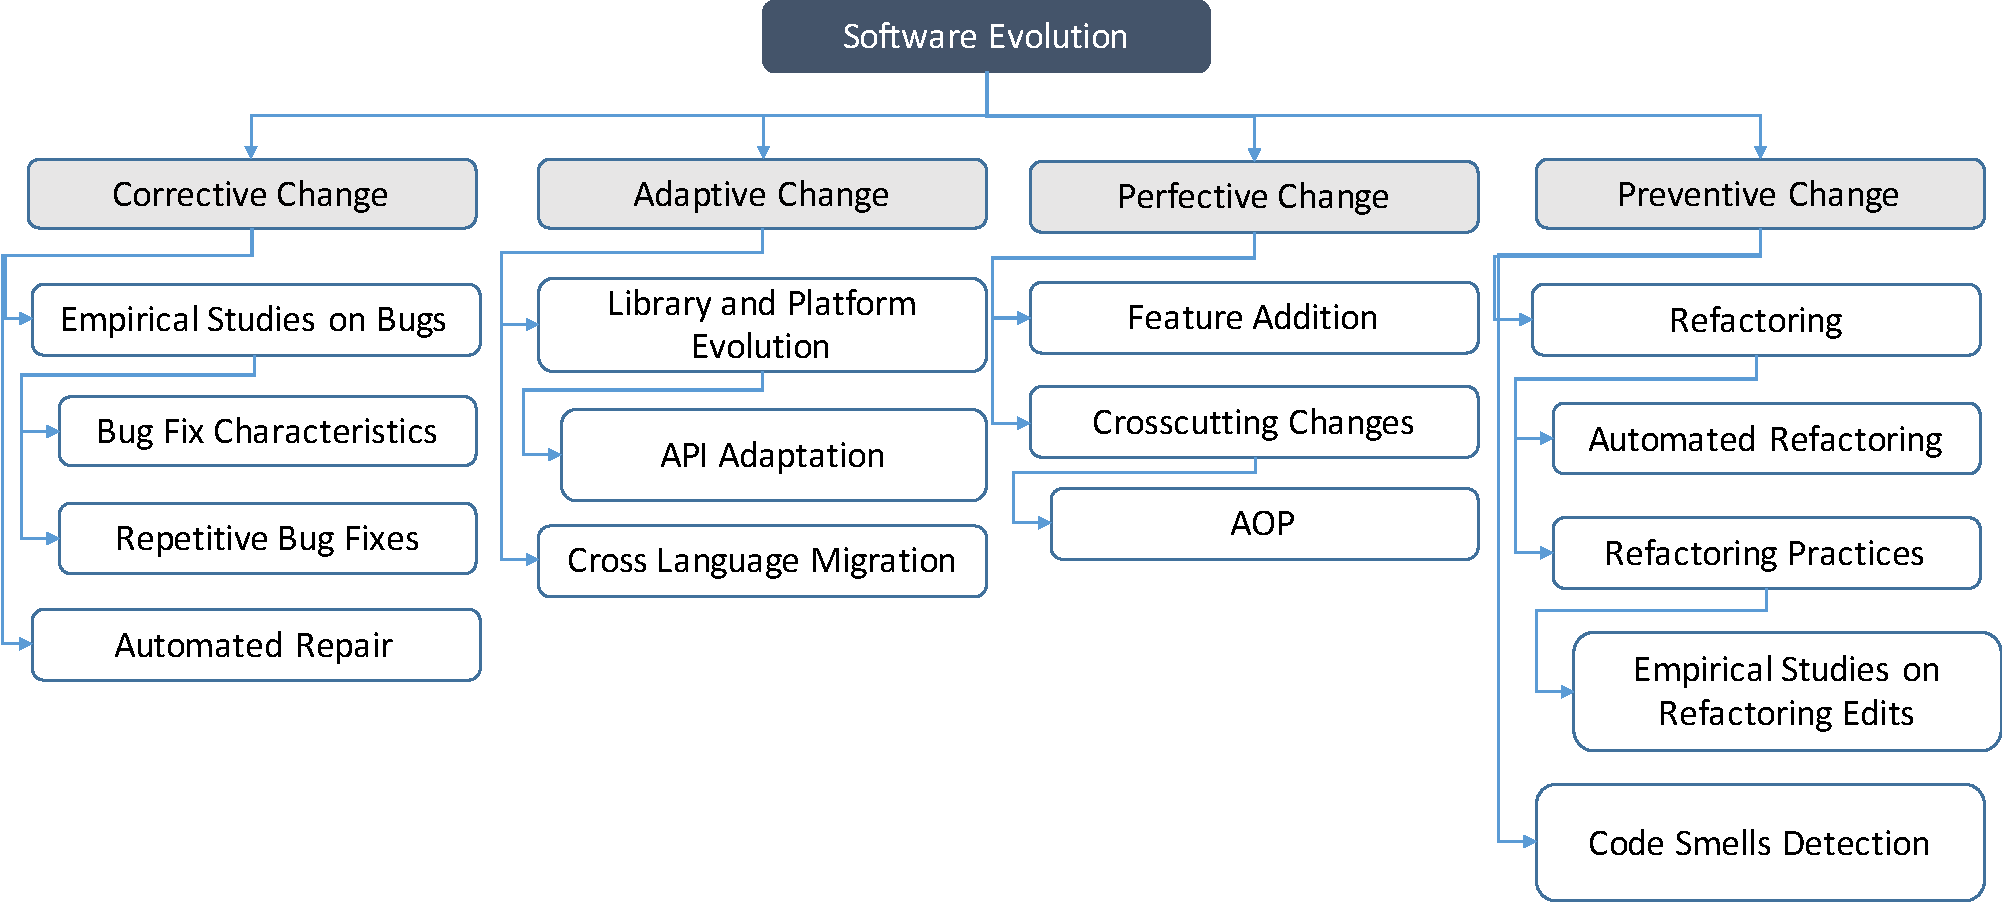
\includegraphics[width=0.95\textwidth]{images/ChangeTypesTopics.pdf}
 \caption{Change Types and Related Research Topics} 
 \label{fig:changetypetopic}
\end{figure}


\subsection{Classifying Software Changes}
\label{sec:classification} 
Swanson initially identified three categories of software changes: corrective, adaptive, and perfective~\cite{Swanson1976:Dimension}. These categories were updated later and ISO/IEC 14764 instead presents four types of changes: corrective, adaptive, perfective, and preventive~\cite{iso}.
\subsubsection{Corrective Change} refers software modifications initiated by software defects. A defect can result from design errors, logic errors, and coding errors~\cite{Longstreet1990:smc}.

\begin{itemize}
\item Design errors: software design does not fully align with the requirement specification. The faulty design leads to a software system that either incompletely or incorrectly implements the requested computational functionality. 
\item Logic errors: a program behaves abnormally by terminating unexpectedly or producing wrong outputs. The abnormal behaviors are mainly due to flaws in software functionality implementations.
\item Coding errors: although a program can function well, it takes excessively high runtime or memory overhead before responding to user requests. Such failures may be caused by loose coding, or the absence of {\em reasonableness checks} on computations performed.
\end{itemize}

\subsubsection{Adaptive Change} is a change introduced to accommodate any modifications in the environment of a software product. The term \textbf{environment} here refers to the totality of all conditions that influence the software product, including business rules, government policies, and software and hardware operating systems. For example, when porting a mobile application from Android to iOS, mobile developers need to apply adaptive changes to translate the code from Java to Swift, so that the software is still compilable and executable on the new platform. Programs may be also changed as a result of a new compiler, which performs additional optimizations to generate smaller and faster code. 

%when maintaining a legacy system that was written in Fortran decades ago, programmers may migrate the system to a mainstream general purpose language, such as Java, to facilitate the maintenance of existing codebase and to extend the system by leveraging new features of the popular language. When building phone apps, Mobile developers may port a mobile application from one platform (e.g., Android) to another (e.g. iOS) by translating code from Java to Swift. 
\subsubsection{Perfective Change} is the change undertaken to expand the existing requirements of a system~\cite{Seaman2008:SMC}. When a software product becomes useful, users always expect to use it in new scenarios beyond the scope for which it was initially developed. Such requirement expansion causes changes to either enhance existing system functionality or to add new features. For instance, an image processing system is originally developed to process JPEG files, and later goes through a series of perfective changes to handle other formats of images, such as PNG and SVG.

\subsubsection{Preventive Change} is the change applied to prevent malfunctions or to improve maintainability of software. 
According to Lehman's laws of software evolution~\cite{Lehman1984:ULE}, the long-term effect of corrective, adaptive, and perfective changes is deteriorating the software structure, while increasing entropy. Preventive changes are usually applied to address the problems. For instance, after developers fix some bugs and implement new features in an existing software product, the complexity of source code can increase to an unmanageable level. Through code refactoring---a series of behavior-preserving changes, developers can reduce the code complexity, and increase both readability and reusability of software.
\begin{figure}[!htb]
\centering
\scalebox{0.5}{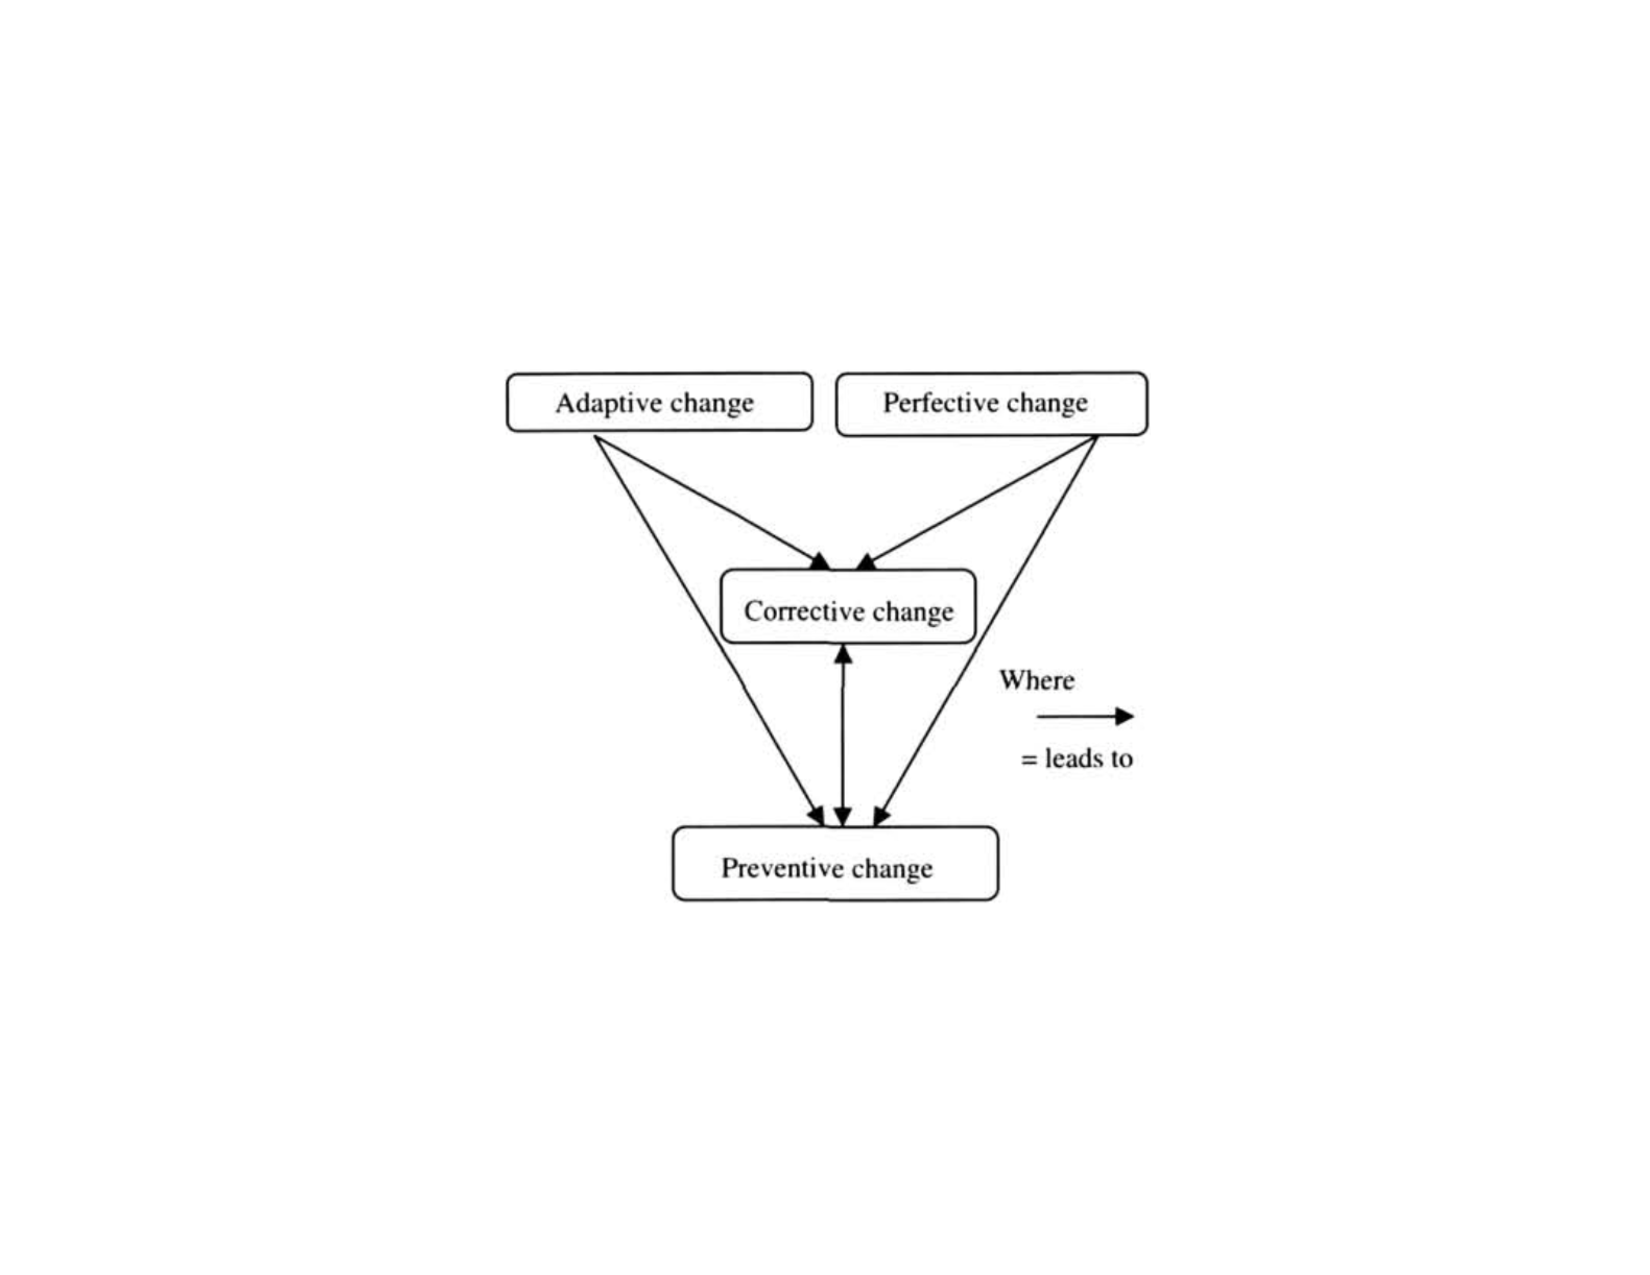
\includegraphics{images/relationship_of_changes.pdf}}
\caption{Potential relation between software changes~\cite{Seaman2008:SMC}}
\label{fig:relation}
\end{figure}

Figure~\ref{fig:relation} presents the potential relationships between different types of changes~\cite{Seaman2008:SMC}. Specifically, both adaptive changes and perfective changes may lead to the other two types of changes, because developers may introduce bugs or worsen code structures when adapting software to new environments or implementing new features.

\subsection{Three Activity Perspectives for Software Changes} 
\label{sec:activity} 
We view the task of evolving software from three activity perspectives: (1) change application, (2) change inspection, and (3) change validation. First, the process of {\em applying} software changes could be further categorized into manual changes vs. automated change application with tool support. In the following three sections, we provide an organized tour of seminal papers focusing on the above-mentioned three kinds of activity perspectives. 

In Section~\ref{sec:apply}, we overview research topics for each of the 4 change types in Section~\ref{sec:classification}. We discuss empirical studies to discuss the characteristics of software changes for each type and overview tool support for applying software changes. For example, for the type of {\em corrective changes}, we present several empirical studies on bug fixes and summarize the characteristics of bug fixes. We then discuss automated techniques for fixing bugs. Similarly, for the type of {\em preventative changes}, we present empirical studies on refactoring practices and refactoring edits and then discuss automated techniques for applying refactorings.  Regardless of change types, various approaches are proposed to reduce the manual effort of updated software through automation. We thus discuss automated change application techniques including source-to-source program transformation, Programming by Demonstration (PbD), simultaneous editing, and systematic editing.

In Section~\ref{sec:inspect}, we overview research topics for inspecting software changes after the corresponding program modifications are made. Software engineers other than the change author perform peer reviews based on their understanding of program changes, and provide feedback if they discover any suspicious software modifications. Therefore, we summarize modern code review processes and discuss techniques for analyzing and understanding code changes. This section overviews a variety of program differencing techniques that developers can use to comprehend code changes and also other types of techniques that raise the abstraction level of program modifications in order to better support the change comprehension and inspection process. 

In Section~\ref{sec:debugtest}, we overview research techniques for validating software changes using debugging, testing, and impact analysis techniques. After software modification is made, developers and testers may create new tests or reuse existing tests based on the requirements specification, run the modified software against the tests, and check whether the software executes as expected. Therefore, the activity of checking correctness about software changes could involve failure-inducing change isolation, regression test selection, and change impact analysis. 


\section{An Organized Tour of Seminal Papers: I. Applying Changes}
\label{sec:apply}
In Sections~\ref{sec:corrective}-\ref{sec:preventive}, for each of the four types of software changes mentioned in Section~\ref{sec:concepts}, we discuss the characteristics of changes using empirical studies, and we also discuss the process and techniques for applying software changes. Next, regardless of change types, automated change application could reduce the effort of applying software changes. Therefore, we discuss the topic of automated program transformation and editing techniques for reducing repetitive edits in Section~\ref{sec:automatic}.

\subsection{Corrective Change}
\label{sec:corrective}
Corrective changes such as bug fixes are frequently applied by developers to eliminate defects in software. There are mainly two lines of research conducted: empirical studies to characterize bugs or corresponding fixes~\cite{Fenton2000:QAF,Li2006:TCE,Kim2006:MBF,Lu2008:LMC,Nguyen2010:RBF,Yin2011:FBB,Park2012:supplementary,Zhong2015:ESR}, and automatic approaches to help developers detect and fix bugs~\cite{Engler2000:CSR,Bush2000:SAF,Hangal2002:TDS,Hovemeyer2004:FBE,Naik2006:ESR,Weimer2009:AFP}. There is no clear boundary between the two lines of research, because some prior work~\cite{Li2006:CPMiner,Pham2010:DRS,Jin2012:UDR,Kim2013:PAR} did leverage the characteristics observed in empirical studies to automatically detect and fix bugs.

\subsubsection{Characterization Studies of Bugs or Fixes}
To analyze bug characteristics, Li et al.~conducted an empirical study on bugs from two popular open source projects: Mozilla and Apache HTTP Server~\cite{Li2006:TCE}. By manually examining 264 bug reports from the Mozilla Bugzilla database~\cite{mozilla}, and 209 bug reports from the Apache Bugzilla database~\cite{asf}, they investigated the root cause, impact, and software components of each software error that exhibited abnormal runtime behaviors. They observed three major root causes: memory, concurrency, and semantics. The memory bugs account for 16.3\% in Mozilla and 12.2\% in Apache. Among memory bugs, NULL pointer dereference was observed as a major cause, accounting for 37.2 to 41.7\%. More importantly, semantic bugs are observed to be dominant, accounting for 81.1\% in Mozilla and 86.7\% in Apache. One possible reason is that most semantic bugs are specific to applications. A developer can easily introduce semantic bugs while coding, due to a lack of thorough understanding of the software. It is challenging to automatically detect or fix such bugs, because diagnosing and resolving them may require a lot of domain-specific knowledge.

To characterize bug fixes, Kim et al.~conduct an empirical study on bug fixing data from the change history of five open source projects: ArgoUML, Columba, Eclipse, jEdit, and Scarab~\cite{Kim2006:MBF}. With keywords like ``Fixed'' or ``Bugs'', they retrieved code commits in software version history that are relevant to bug fixes, chopped each commit into contiguous code change blocks (i.e., hunks), and then clustered similar code changes. They observed that 19.3 to 40.3\% bugs appeared repeatedly in version history, while 7.9 to 15.5\% of bug-and-fix pairs appeared more than once. The results demonstrate that project-specific bug fix patterns occur frequently enough to be useful as a bug detection technique. Furthermore, for the bug-and-fix pairs, it is possible to both detect the bug and provide a strong suggestion for the fix. 

\begin{table}[]
\centering
\caption{Sample system rule templates and examples from~\cite{Engler2000:CSR}}
\label{tab:rule}
\begin{tabular}{l|l}
\toprule
Rule template                  & Example                                                 \\ \hline
``Never/always do X''          & ``Do not use floating point in the kernel''             \\\hline
``Do X rather than Y''         & ``Use memory mapped I/O rather than copying''           \\ \hline
``Always do X before/after Y'' & ``Check user pointers before using them in the kernel''\\
\bottomrule
\end{tabular}
\end{table} 

\subsubsection{Automatic Bug Detection and Fixing Approaches for Software Evolution} 
Engler et al.~defined a meta-language for users to easily specify temporal system rules such as ``release locks after acquiring them''~\cite{Engler2000:CSR}. They also extended a compiler to interpret the rules and dynamically generate additional checks in the compiler. If any code snippet violates the specified rule(s), the approach reports the snippet as a software bug. Table~\ref{tab:rule} presents some exemplar system rule templates and instances. 
With this approach, developers can flexibly define their own rules to avoid some project-specific bugs, without worrying how to implement checkers to enforce the rules.

Li et al. developed CP-Miner, an automatic approach to find copy-paste related bugs in large-scale software~\cite{Li2006:CPMiner}. CP-Miner was created based on a prior empirical study~\cite{Chou2001:ESO}, which revealed that under the Linux {\sf drivers/i2o} directory, 34 out of 35 errors were caused by copy-paste or duplicated code. 
One of the major reasons why copy-paste introduces bugs is that when developers copy code from one location and paste it to another location, they forget to consistently rename identifiers of variables, functions, and types. CP-Miner first identifies copy-paste code in a scalable way, and then detects bugs associated with copy-paste by checking the renamed identifiers. If an identifier is inconsistently renamed, with some of its occurrences replaced and some not replaced, CP-Miner reports it as a copy-paste bug. Many previously unknown bugs in popular operating systems were detected in this way, 49 in Linux and 31 in FreeBSD, meaning that CP-Miner can effectively capture copy-paste related bugs. 
 
\subsection{Adaptive Change}
\label{sec:adaptive}
Adaptive changes are applied to a software product, when its environment changes. In this section, we focus on two scenarios when adaptive changes are applied: software library upgrade and cross-language software migration.
\todo{Na, don't we need to describe changes coming from environment changes more broadly? I think it would make sense to include a category of feature addition. It seems to be the two categories of library update and cross-language transformation seem too narrow in its focus and not comprehensive enough to describe various kinds of software changes. Could we add a new category of platform update, changes to improve performance, etc?} 


\subsubsection{Software Library Upgrade} 
When building new software (e.g., a search engine), instead of coding everything from scratch, developers always extend existing frameworks or third-party libraries (e.g., Lucene~\cite{lucene}) by invoking the Application Programming Interfaces (APIs), to reuse the well implemented and fully tested functionality. However, as library developers release new versions of their software to fix existing bugs and include new features, client developers should also upgrade the libraries used in their projects to benefit from the newer versions. Ideally, the library APIs should be stable so that such software upgrades do not incur any program change in client applications. In reality, nevertheless, these APIs are susceptible to changes, requiring client developers to apply adaptive changes for the usage of new library versions. 

\begin{figure}
\centering
\scalebox{0.4}{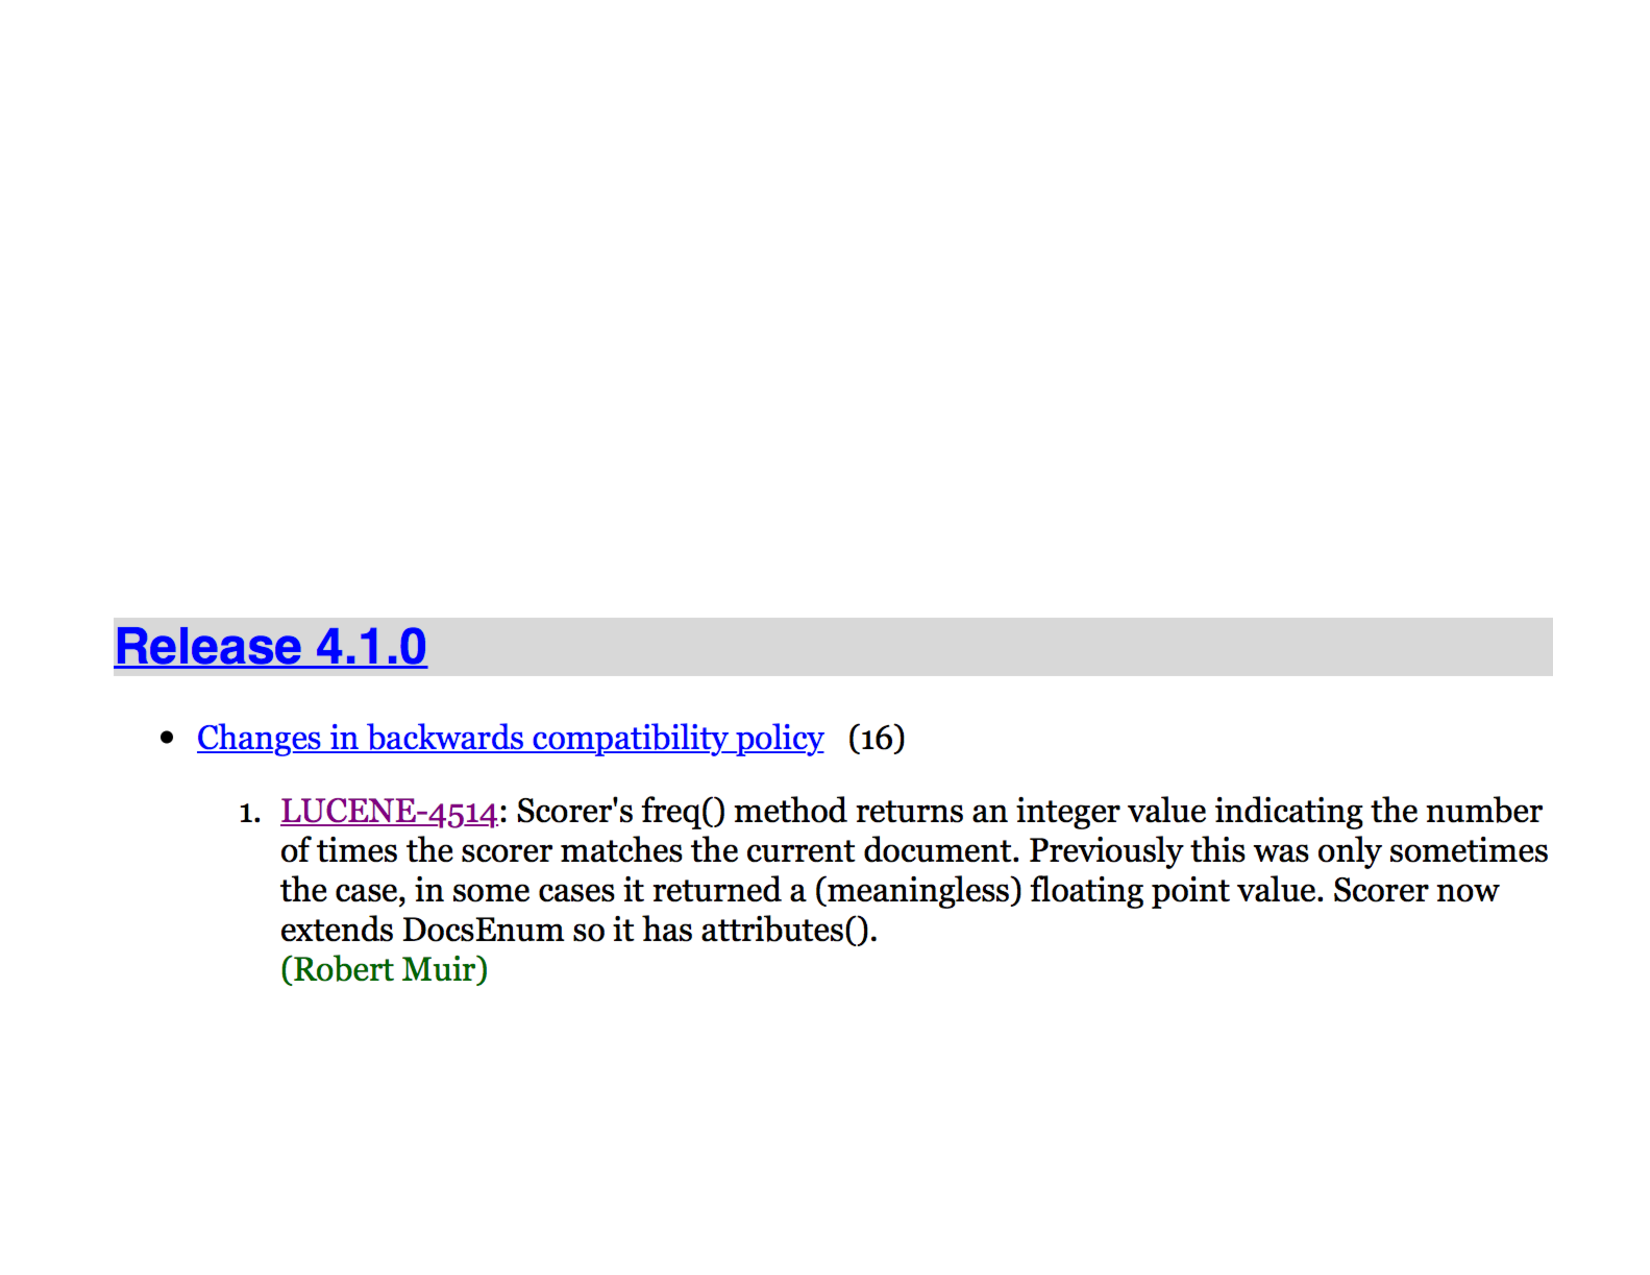
\includegraphics{images/releasenote.pdf}}
\caption{An excerpt of the Lucene change log for Release 4.1.0~\cite{releasenote}}
\label{fig:releasenote}
\end{figure}

\todo{Na, while the following text makes the text and example very concrete, I think it is too pertinent to a particular project and it is unclear what is the take away message that you want to say about the nature of software library upgrade.} 
Figure~\ref{fig:releasenote} presents an excerpt of the Lucene change log for Release 4.1.0~\cite{releasenote}. According to the release note, there are 16 recent changes in the library that can make client applications incompatible with the new release, requiring client developers to manually resolve the issues. Among the 16 changes, the first one is about a return type change of Scorer's \codefont{freq()} method. Previously, the method returns a float number, and now it returns an integer. Correspondingly, client code should be changed to properly process the new values returned by this method. By manually checking such release notes and searching for candidate solutions online, client developers can apply adaptive changes to solve any incompatibility issues between client code and new library releases.

Researchers proposed approaches to automatically infer and recommend such adaptive changes for framework or library evolution~\cite{Dagenais2008:RAC,Schafer2008:MFU,Zhong2009:MMR,Wu2010:AHA,Nguyen2010:GAA}. For instance, Dagenais et al.~developed SemDiff, an automatic approach that compares two releases of a library or framework to infer any adaptive change of API replacements~\cite{Dagenais2008:RAC}. 
\todo{Na, the example appearing here fore API migration seems very toy-like example and also in terms of evolution types, it seems too trivial and narrowly focused. Is it possible to update the following text?}  
Suppose in the old library release, there are two methods: \codefont{caller1} and \codefont{caller2}, both of which invoke a library public API \codefont{m1()}. However, in the new library release, both methods instead invoke another public API \codefont{m2()}. Therefore, SemDiff infers an API replacement pattern \codefont{m1()->m2()}. When scanning a client application built on the old library release, SemDiff automatically recommends the inferred adaptive change for every invocation of \codefont{m1()}.

\subsubsection{Cross-language Software Translation}
When maintaining a legacy system that was written in an old programming language (e.g., Fortran) decades ago, programmers may migrate the system to a mainstream general-purpose language, such as Java, to facilitate the maintenance of existing codebase and to extend the system by leveraging new features of the popular language. Different from the API adaptive changes mentioned above, such software translation requires of a significant amount of coding effort to rewrite the same application in a new programming language.

\todo{Na, could we move this part on TXL to Section 3.5 on automated change application? In my opinion is a TXL is a general program transformation technique and is more than cross-language software translation.} 

TXL is a source transformation language designed to translate or manipulate programming languages~\cite{Cordy2006}. As shown in Figure~\ref{fig:txl}, a typical TXL file consists of two parts. The first part defines a context-free grammar to describe program syntax, while the second part describes a set of transformation rules to manipulate the syntax. For our illustrative example, the grammar defines a simple language that only allows numbers, addition and subtraction numerical expressions. The rule \codefont{resolveAddition} describes the resolution of an addition expression by replacing the expression with a number value \codefont{N1 [ + N2 ]}. Given such a file, the TXL program transformation engine automatically transforms programs of the syntactic structure by applying the rules. 
%However, manually defining translation rules using this domain-specific language is still cumbersome and error-prone for developers.

\begin{figure}
\centering
\scalebox{0.5}{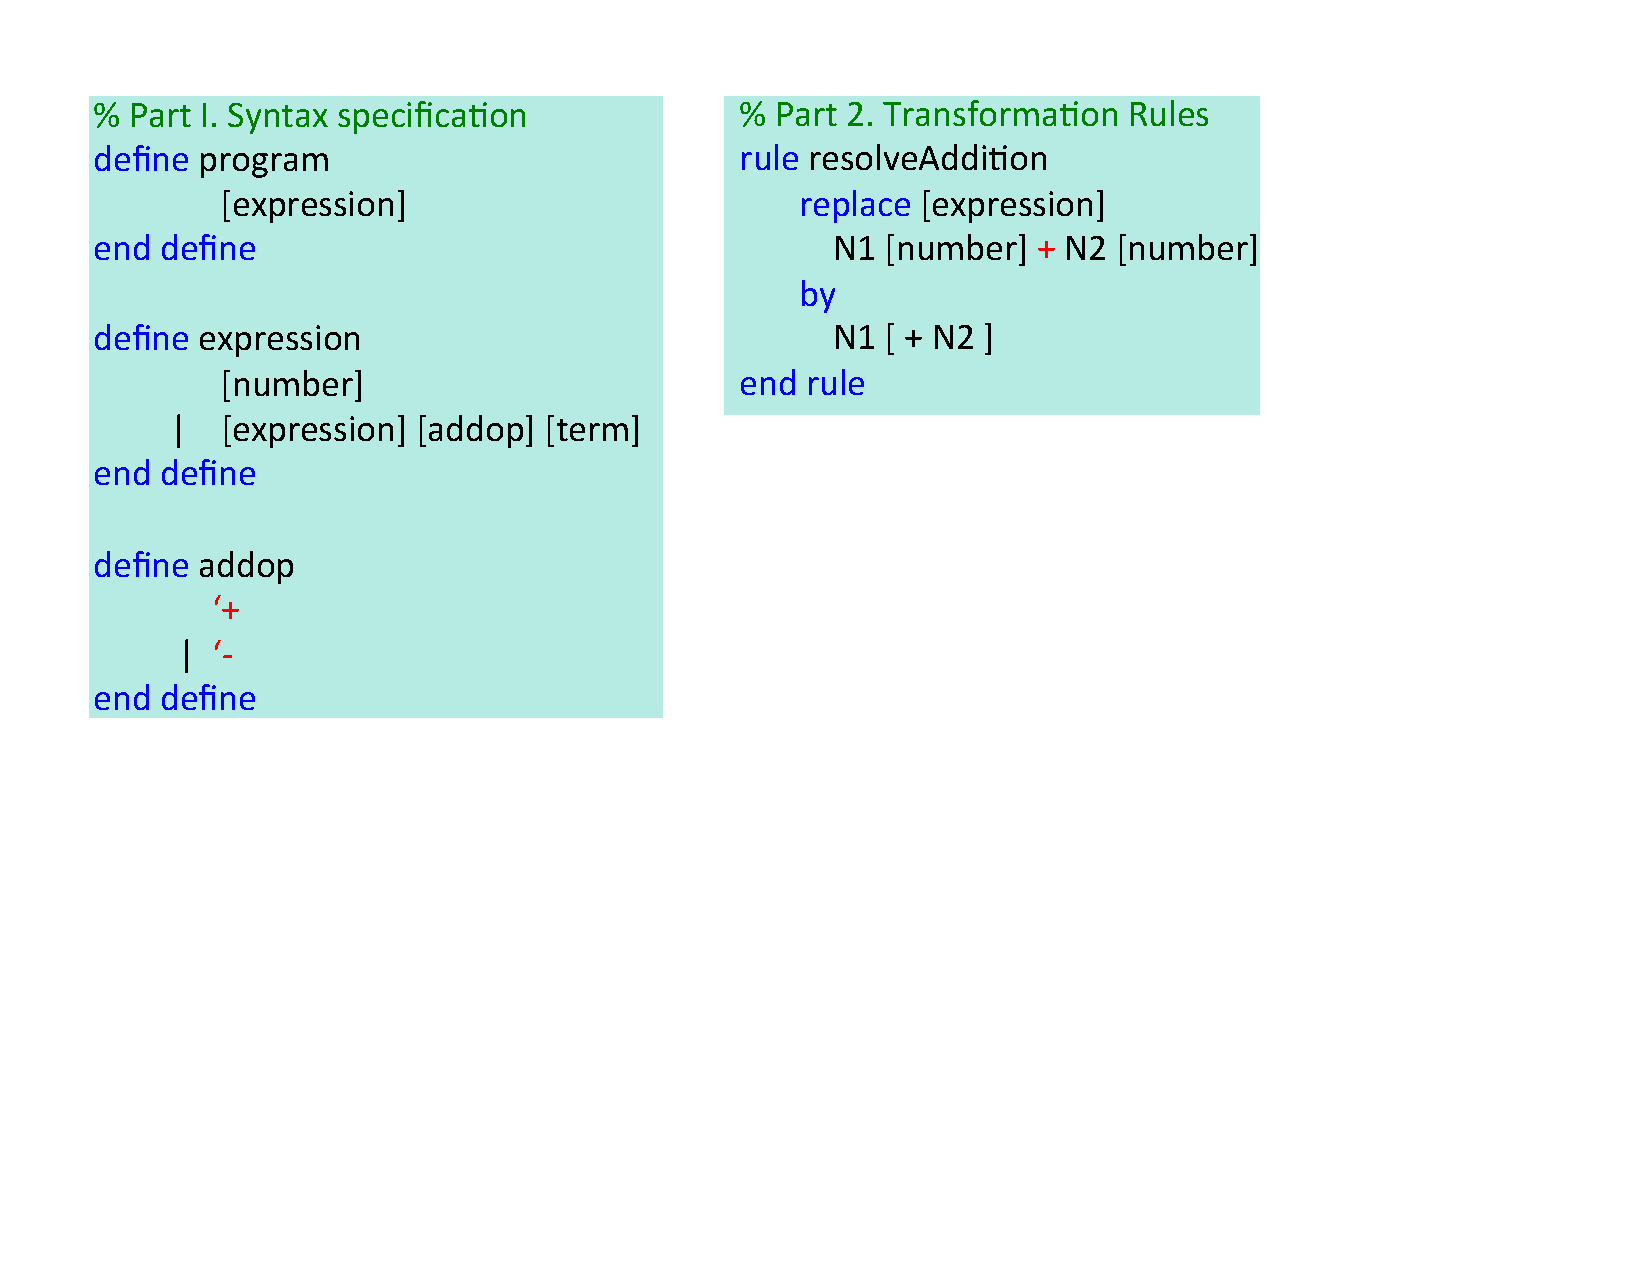
\includegraphics{images/txl.pdf}}
\caption{A simple exemplar TXL file based on~\cite{txltour}}
\label{fig:txl}
\end{figure}
With TXL, developers to not need to build programming language translators by coding every line of implementation. Instead, the transformation engine can automatically translate code once developers specify all needed grammars and rules. Researchers built tools using TXL to automate various code translation tasks, like ASP-to-NSP and Java-to-C\#~\cite{Chu:08,Hassan:2005,El-Ramly:2006,Tonella:04}.
%For instance, Hassan et al. migrated web applications between different web development frameworks like ASP and NSP~\cite{Hassan:2005}, while El-Ramly et al.~converted Java programs to C\#~\cite{El-Ramly:2006}. 

\todo{Na, again I feel that we need a broader discussion on adaptive changes.} 

\subsection{Perfective Change}
\label{sec:perfective}
\todo{Isn't the perfective change a refactoring? I think the below problem of crosscutting concerns seem to be in the category of adaptive or additive changes to me. I suggest us to move the crosscutting concerns to the previous sub section and write about refactorings broadly here.} 
Developers apply perfective changes when enhancing or adding software features by implementing new code. There is not much research done in this area to facilitate feature enhancement or addition. One possible reason is that the implementation logic is always project-specific and spontaneous. It is challenging for any automatic tool to predict what new code to add, and to suggest what rules to apply when integrating new code with existing codebases. In this section, we mainly focus on two most closely relevant research topics: Aspect Oriented Programming (AOP) and Feature Oriented Programming (FOP).

\todo{Na, could you please write about the properties / characteristics of cross-cutting concerns and why cross-cutting concerns appear, before describing an AOP and FOP. In other words, I think we need to define a problem first, before discussing techniques/ solutions.} 

\subsubsection{AOP} is a programming paradigm that aims to increase modularity by allowing the separation of cross-cutting concerns~\cite{Kiczales1997}. Suppose developers want to add a new feature---logging---to log all executed functions. 
The logging logic is straightforward: printing the function's name at each function's entry. However, manually inserting the same implementation to each function body is tedious and error-prone. With AOP, developers only need to first define the logging logic as \textbf{an advice}, and then specify the place where to insert the advice (i.e., \textbf{pointcut}), such as the entry point of each function. An aspect weaver will read the aspect-oriented code, and generate appropriate object-oriented code with the aspects integrated. In this way, AOP facilitate developers to efficiently introduce new program behaviors without cluttering the core implementation in the existing codebase. Many Java bytecode manipulation frameworks implement the AOP paradigm, like ASM~\cite{asm}, Javassist~\cite{javassist}, and AspectJ~\cite{aspectj}, so that developers can easily modify program runtime behaviors without touching the source code. 


\subsubsection{FOP} is a paradigm for program generation in software product lines and for incremental development of programs~\cite{Batory1992:DIH}. 
FOP is closely related to AOP. Both deal with modules that encapsulate crosscuts of classes, and both express program extensions.
In FOP, every software is considered as a composition of multiple features or layers. Each feature implements a certain program functionality, while features may interact with each other to collaboratively provides a larger functionality or get adapted to each other.
A software product line (SPL) is a family of programs where each program is defined by a unique composition of features. Formally, FOP considers programs as \emph{values} and program extensions as \emph{functions}~\cite{Lammel2013:fop}. Suppose there are two programs: 

$f \text{	// program with feature }f$, and

$g\text{	// program with feature }g$.

\noindent
A program extension is a function that takes a program as input and produces a feature-augmented program output. Suppose there are two program extensions:

$i \bullet x$ // adds feature i to program x, and 

$j \bullet y$ // adds feature j to program y.

By applying the functions to the values, we can compose more than one multi-featured application as below:

$app1 = i \bullet f$ // app1 has features i and f,

$app2 = j \bullet g$ // app2 has features j and g, and
 
$app3 = i \bullet j \bullet f$ // app3 has features i, j, f.

\subsection{Preventive Change}
\todo{Na, I suggest to combine preventive and perfective changes together, since it is not clear to me how they are really different, and refactoring seems to belong both the categories of preventive and perfective changes. } 

\label{sec:preventive}
Program refactorings~\cite{Fowler1999:refactoring} are usually conducted to increase software maintainability, readability, or reliability, and to prevent problems in future. \todo{Na,  I wish we have much broader discussion of refactoring.} Opdype defines that a refactoring is behavior-preserving, if given the same set of input values, a program always produces the same set of output values before and after the refactoring~\cite{Opdyke1992:ROF}. Fowler et al.~introduced 71 code refactorings that developers can apply to their code, and summarized why and how to apply each refactoring~\cite{Fowler1999:refactoring}. Typically, a refactoring process consists of the following activities~\cite{Mens2004:SSR}:
\begin{enumerate}
\item Identifying where to apply what refactoring(s).
\item Checking that the refactoring to apply preserves program behaviors.
\item Refactoring the code.
\item Assessing the effect of applied refactoring on software quality (e.g., complexity and readability). 
\item Maintaining the consistency between refactored code and other related software artifacts, like documentation, tests, and issue tracking records.  
\end{enumerate}

Researchers have proposed different approaches, techniques, or formalisms to support each of above activities.

\subsubsection{Identifying Where to Apply What Refactorings}
Various approaches have been proposed to automatically suggest refactoring opportunities based on program context, code smells, or version history~\cite{Balazinska2000:ACA,Kataoka2001:ASP,Higo2008:metricrefactoring,Tsantalis2011:rankRefactoring,Wang2014:recommendClones,Meng2015:ARO}. Specifically, Kataoka et al.~developed Daikon to infer program invariants at runtime, and thus to suggest candidate refactorings~\cite{Kataoka2001:ASP}. For instance, if Daikon observes that one parameter of a method is always constant, it then suggests a \emph{removeParameter} refactoring. Balazinska et al.~used a clone detection tool to identify duplicated code and to suggest clone removal refactorings~\cite{Balazinska2000:ACA}. Tsantalis et al.~ranked clones that have been repetitively or simultaneously changed in the past to suggest refactorings~\cite{Tsantalis2011:rankRefactoring}. Wang et al.~extracted features from code to reflect program context, code smell, and evolution history, and then used a machine learning technique to rank clones for refactorings~\cite{Wang2014:recommendClones}.

\subsubsection{Checking the Behavior-Preserving Property of Refactorings}Opdyke suggested to ensure such behavior preservation by specifying \emph{refactoring preconditions}~\cite{Opdyke1992:ROF}. For instance, when conducting an \emph{create\_method\_function} refactoring, before inserting a member function $F$ to a class $C$, developers should specify and check for five preconditions, as shown in Figure~\ref{fig:preconditions}. If any precondition is not satisfied, the refactoring should not be applied to the program.

\begin{figure}[!htb]
\centering
\scalebox{0.55}{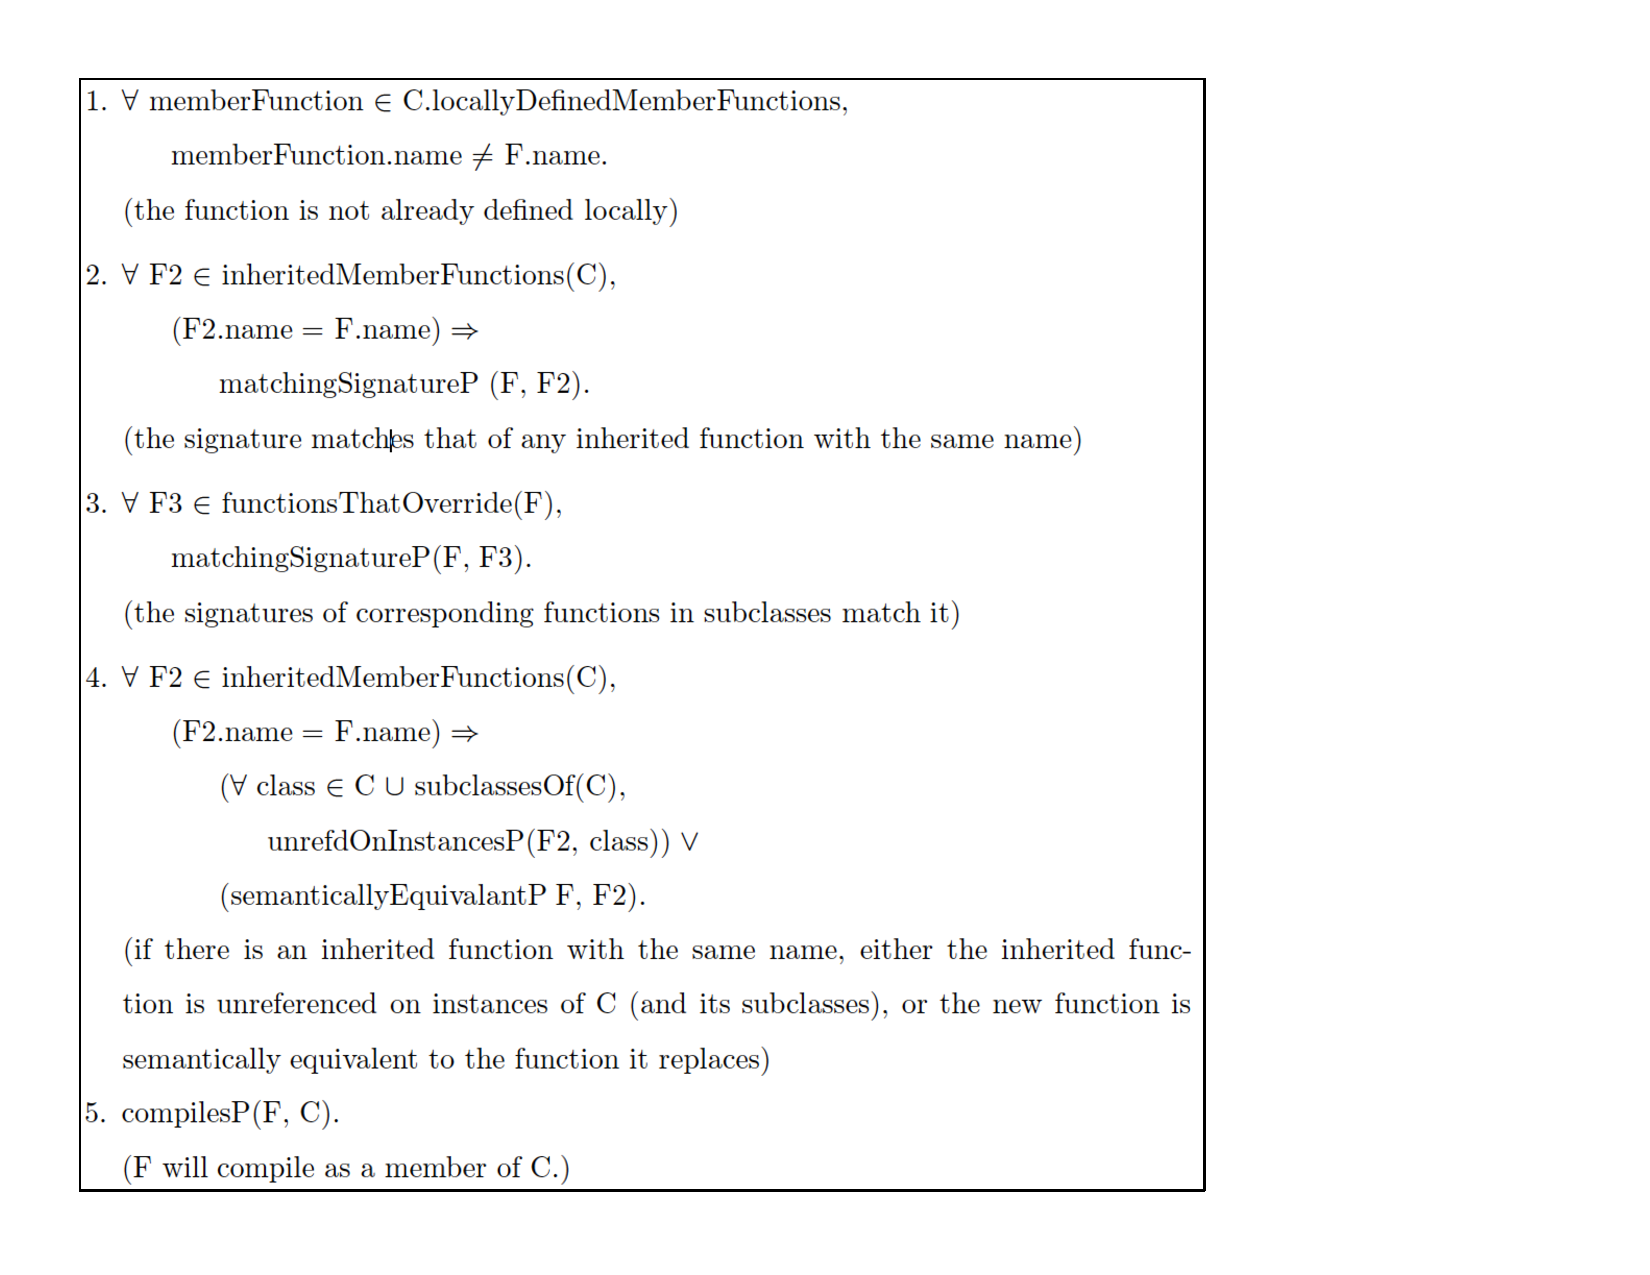
\includegraphics{images/preconditions.pdf}}
\caption{Preconditions for \emph{create\_method\_function} refactoring~\cite{Opdyke1992:ROF}}
\label{fig:preconditions}
\end{figure}

\subsubsection{Applying Refactorings}
The Eclipse IDE provides automatic support for a variety of refactorings, including \emph{rename}, \emph{move}, and \emph{extractMethod}. With such support, developers do not need to worry about how to check for preconditions or postconditions before manually applying a certain refactoring. Instead, they can simply select the refactoring command from a menu (e.g., \emph{extractMethod}), and provide necessary information to accomplish the refactoring (e.g., method name). The Eclipse refactoring engine takes care of the precondition check, program transformation, and postcondition check. Additionally, 
researchers conducted empirical studies to characterize the refactorings applied by developers~\cite{Kim2012:FSR,Murphy-Hill2012:refactor,Vailian2012:misuse,Silva2016:WWR}, and proposed various approaches to automate refactoring or to complete the refactoring tasks initiated by developers~\cite{Griswold:1992,Balazinska1999,Dig:2009,Ge:2012,Chen:2013,Lee:2013,Tsantalis2013:icsm,Meng:2015,Kim:2016}. For instance, Silva et al.~observed that refactoring activity is mainly driven by changes in the requirements and much less by code smells~\cite{Silva2016:WWR}. Kim et al.~developed R3, an alternative refactoring engine that works 10 times faster than Eclipse Refactoring~\cite{Kim:2016}. 

\subsubsection{Assessing the Effect of Refactoring} 
To understand whether any refactoring application actually improves software quality, researchers proposed 
different techniques to measure the impact of refactorings~\cite{Kataoka2002:evaluateRefactor,Tahvildari2003:MAE}. Specifically, Kataoka et al.~proposed coupling metrics to evaluate the refactoring effect~\cite{Kataoka2002:evaluateRefactor}. By comparing the coupling before and after the refactoring, they assessed the degree of maintainability enhancement. Similarly, Tahvildari et al.~suggested using a catalogue of object-oriented metrics to estimate refactoring impact, including complexity metrics, coupling metrics, and cohesion metrics~\cite{Tahvildari2003:MAE}. 
\todo{write about Microsoft study and Kim et al.} 


\subsubsection{Maintaining Consistency of Refactored Software} 
Approaches were investigated to ensure the consistency between refactored programs and other software artifacts like design models~\cite{Bottoni2003:coordinatedTransformation,Straeten2003:UML}. For example, Bottoni et al.~modeled a refactoring as a set of distributed graph transformations~\cite{Bottoni2003:coordinatedTransformation}. Each time a code refactoring is applied, the corresponding graph transformations are automatically applied to related design models to preserve consistency. Van Der Straeten et al.~suggested using description logic to maintain the consistency between relevant UML models as they evolve~\cite{Straeten2003:UML}.


\subsection{Automatic Change Application}
\label{sec:automatic}


\begin{figure}[ht]
 \centering
 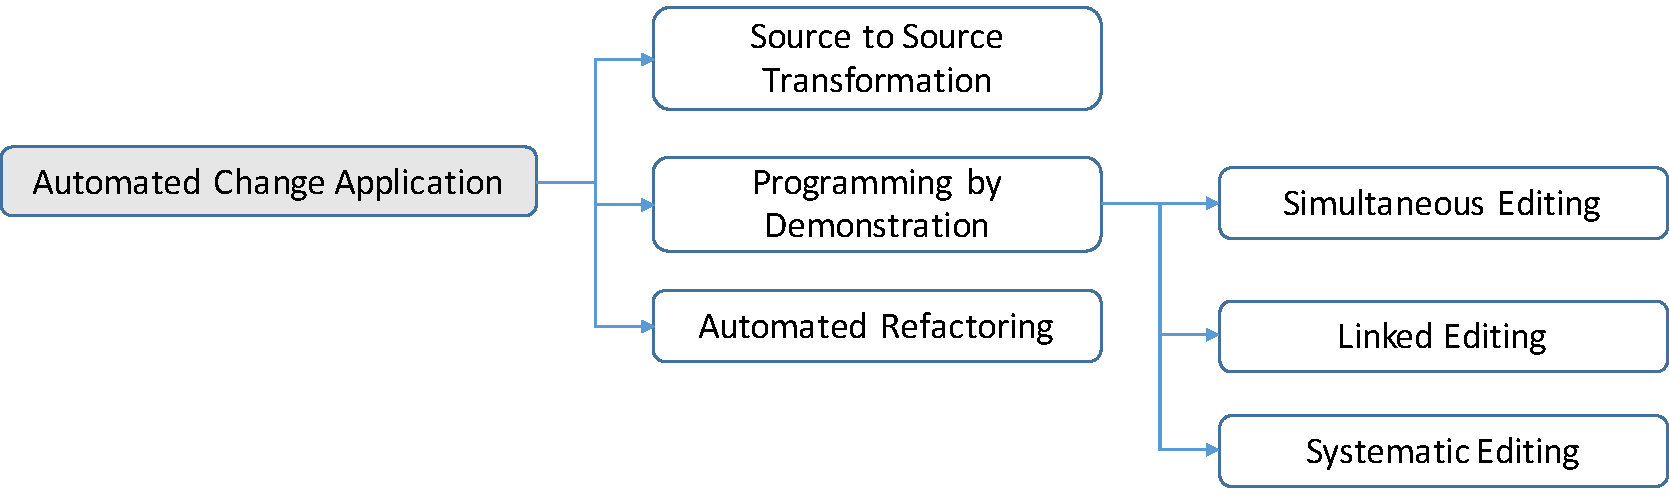
\includegraphics[width=0.95\textwidth]{images/AutomatedChange.pdf}
 \caption{Automated Change Application and Related Research Topics} 
 \label{fig:automaticapplication} 
\end{figure}



Regardless of change types, various approaches are proposed to automatically suggest program changes to developers or reduce the manual effort of updating software. In this section, we discuss automated change application techniques including source-to-source program transformation, Programming by Demonstration (PbD), simultaneous editing, and systematic editing.

\todo{I think we need to write about S2S program transformation more broadly here.} 

\subsubsection{PbD} is also called Programming by Example (PbE). It is an end-user development technique for teaching a computer or a robot new behaviors by demonstrating the task to transfer directly instead of manually programming the task.
Approaches were built to generate programs based on the text-editing actions demonstrated or text change examples provided by users~\cite{Nix1984,WiM1993,LaH1995,LWD2001}. For instance, 
TELS records editing actions such as search-and-replace, and generalizes them into a program that transforms input to output~\cite{WiM1993}. It leverages heuristics to match actions against each other to detect any loop in the user-demonstrated program. 
Similarly, SMARTedit~\cite{LWD2001} automates repetitive text-editing tasks by learning programs to perform them using techniques drawn from machine learning. SMARTedit represents a text-editing program as a series of functions that alter the state of the text editor (i.e., the contents of the file, or the cursor position). Like macro recording systems, SMARTedit learns the program by observing a user performing her task. However, unlike macro recorders, SMARTedit examines the context in which the user's actions are performed and learns programs that work correctly in new contexts. 

\subsubsection{Simultaneous Editing} repetitively applies source code changes that are interactively demonstrated by users~\cite{MiM2001}. When users apply their edits in one program context, the tool replicates the \emph{exact lexical} edits to other code fragments, or transforms code accordingly. For instance, Linked Editing requires users to first specify the similar code snippets which they want to modify in the same way~\cite{TBG2004}. As users interactively edit one of these snippets, Linked Editing simultaneously applies the identical edits to other snippets. 
CloneTracker takes the output of a clone detector as input and creates a descriptor for each clone~\cite{DuR2007}. With such descriptors, CloneTracker tracks clones across program versions and identifies any modification to those clones. 
Similar to Linked Editing, CloneTracker also echoes edits in one clone to other counterparts upon a developer's request. 
Clever is another clone management system that tracks code clone groups and detects any inconsistent change applied to clones within the same group~\cite{NNP2009}. If a clone misses the updates applied to the other clones in the same group, Clever automatically suggests the missing update to that clone.

\subsubsection{Systematic Editing} is the process of applying similar, but not necessarily identical, program changes to multiple code locations. 
%Prior work shows that programmers apply systematic edits to either add features, fix bugs, or refactor code~\cite{Kim:2005,Kim:2009,Nguyen:2010}. 
Manually applying systematic edits is tedious and error-prone. 
%for two reasons. 
%First, developers may forget to apply systematic edits to all program contexts where the edits are needed, committing errors of omission. Second, developers may apply edits inconsistently and thus introduce new bugs. 
%To improve programmer productivity and software quality, 
Several approaches~\cite{MKM2011,MKM2013,Rolim:2017} have been proposed to infer the general program transformation from one or more code change examples provided by developers, and then apply the transformation to other program contexts in need of similar changes. Specifically, LASE requires developers to provide multiple similarly changed Java methods (at least two)~\cite{MKM2013}. By extracting the commonality between demonstrated changes and abstracting the changes in terms of identifier usage and control- or data-dependency constraints in edit contexts, LASE creates a general program transformation, which can both detect code locations that should be changed similarly, and suggest customized code changes for each candidate location.





\paragraph{Refactoring Practices} 
\todo{1 page: Write the following paragraph more broadly. refactoring is a special category of automated transformation: refactoring practices (kim et al., emerson murphy hill, ralph johnson) } 
Code refactoring is the process of restructuring source code without changing its external behaviors. It is usually applied to improve code readability or extensibility, or to reduce code complexity. 
Fowler et al.~defined a catalog of refactorings that developers can apply to improve their codebase in different ways~\cite{1999:RID}, although developers can also define and manually apply their own refactorings. Eclipse IDE also provides tool support to automate some of the refactorings mentioned in Fowler's catalog, such as \emph{Extract Method}, \emph{Pull up Method}, and \emph{Move Field}. Researchers proposed various approaches to automate refactoring or to complete the refactoring tasks initiated by developers~\cite{Griswold:1992,Balazinska1999,Dig:2009,Ge:2012,Chen:2013,Lee:2013,Tsantalis2013:icsm,Meng:2015,Kim:2016}.

\section{An Organized Tour of Seminal Papers: II. Inspecting Changes}
\label{sec:inspect}

\begin{figure}[ht]
 \centering
 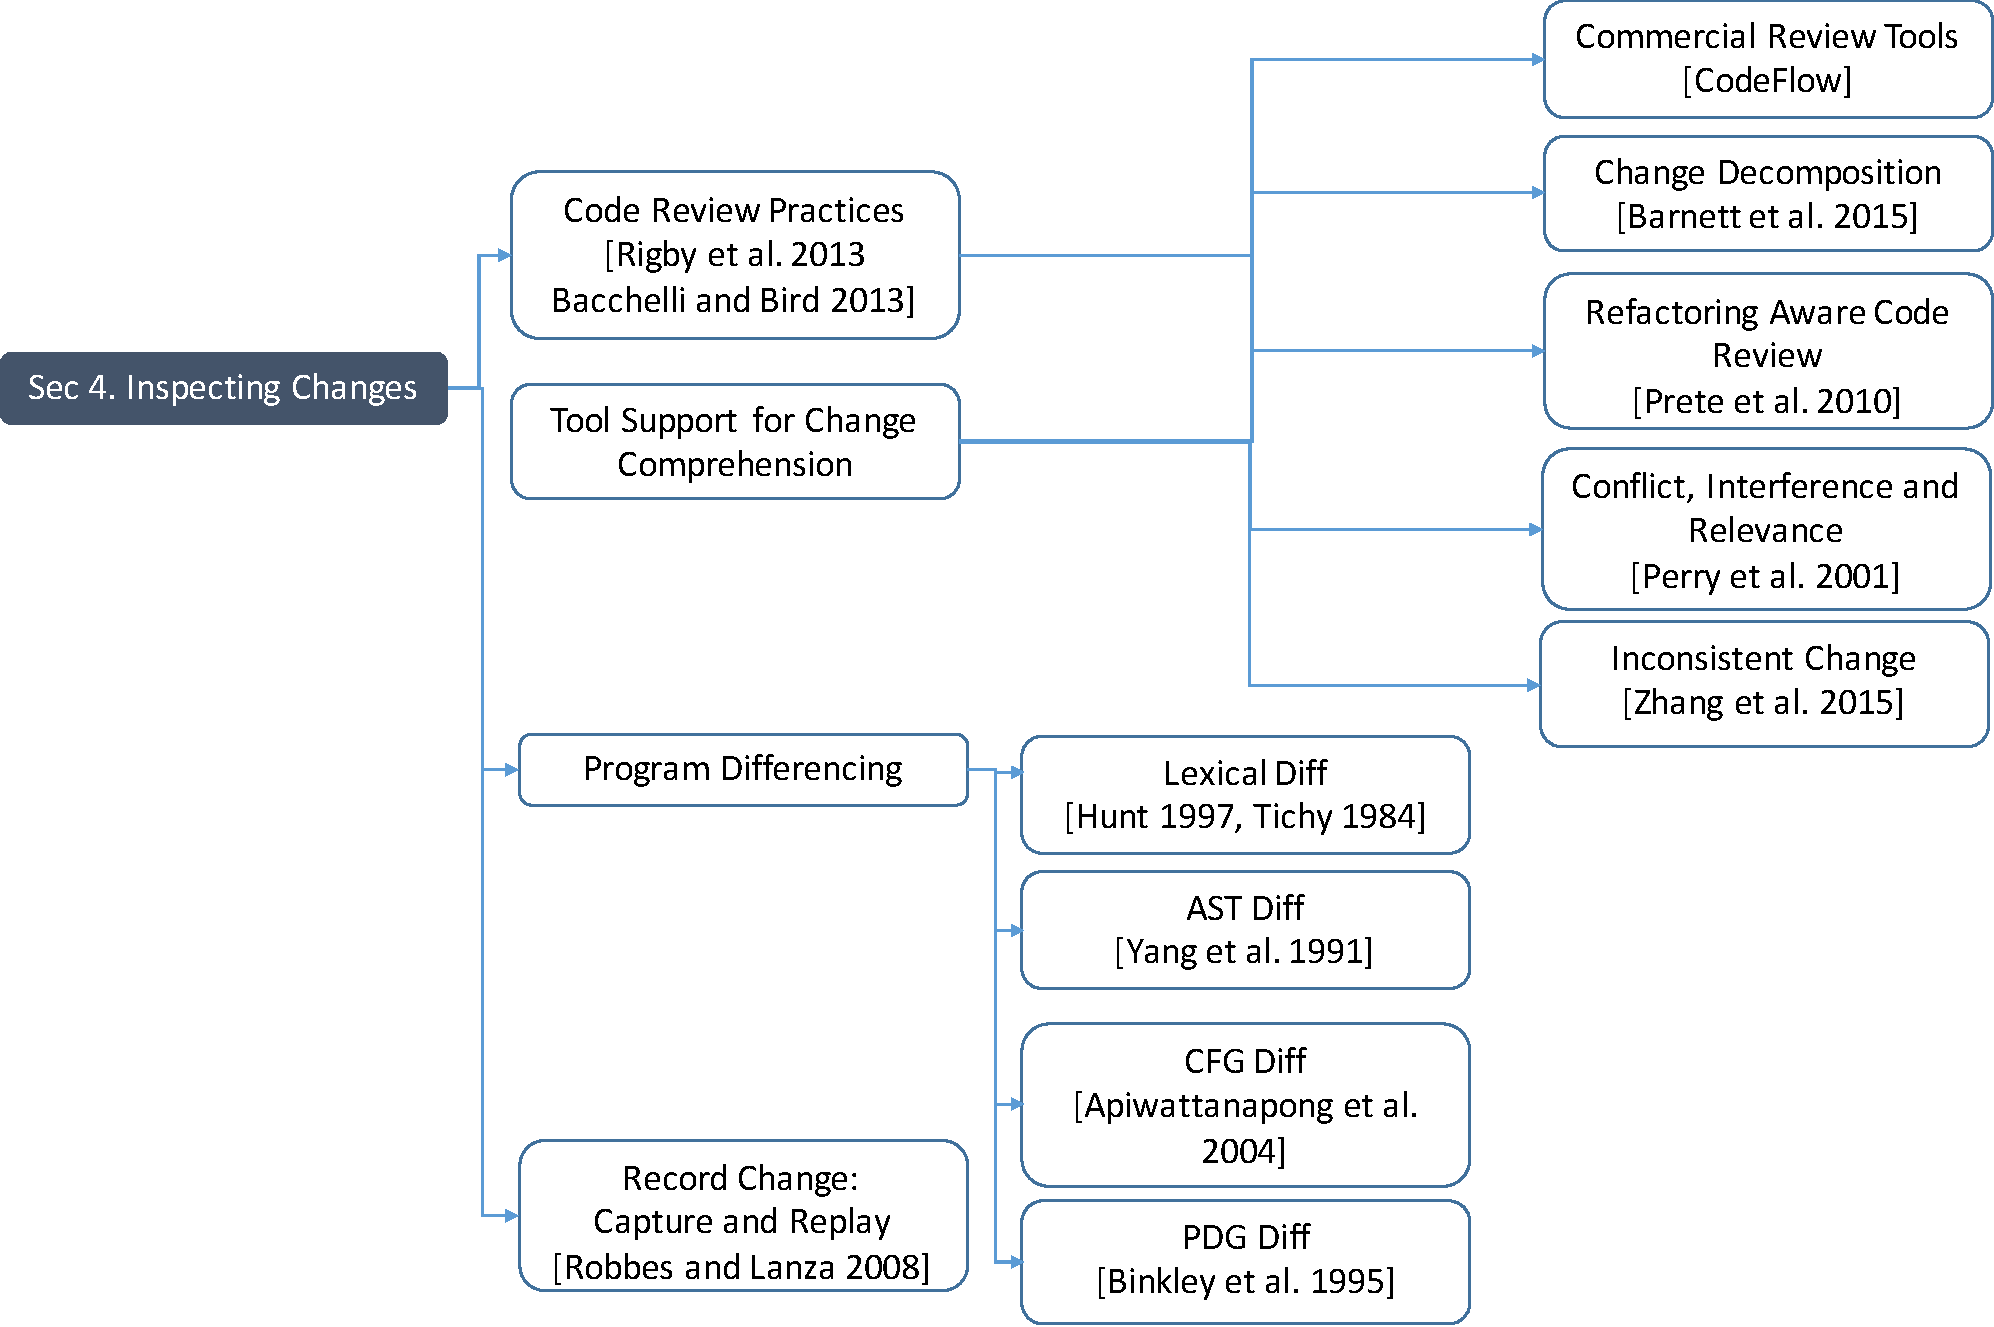
\includegraphics[width=0.95\textwidth]{images/ChangeInspection.pdf}
 \caption{Change Inspection and Related Research Topics} 
 \label{fig:changeinspection} 
\end{figure}

\todo{8 pages- Tianyi is in charge} 
\subsection{Code Review Practices}
To improve the correctness and quality of software systems, developers often perform {\em code review} to manually examine program changes made to software systems. Michael Fagan from IBM first introduced ``code inspections'', the original name of code review, in a seminal paper in 1976~\cite{fagan2001design}. Code inspections are performed at the end of major software development phases, with the aim of finding overlooked defects before moving to the next phase. Software artifacts are circulated a few days in advance and then reviewed and discussed in a series of meetings. The meetings include the author of an artifact, other developers to assess the artifact, a meeting chair to moderate the discussion, and a secretary to record the discussion. Over the years, code inspections have been proven a valuable method to improve  software quality. However, the cumbersome and time-consuming nature of code inspections hinders its adoption in practice~\cite{johnson1998reengineering}. 

\begin{figure}[ht]
 \centering
 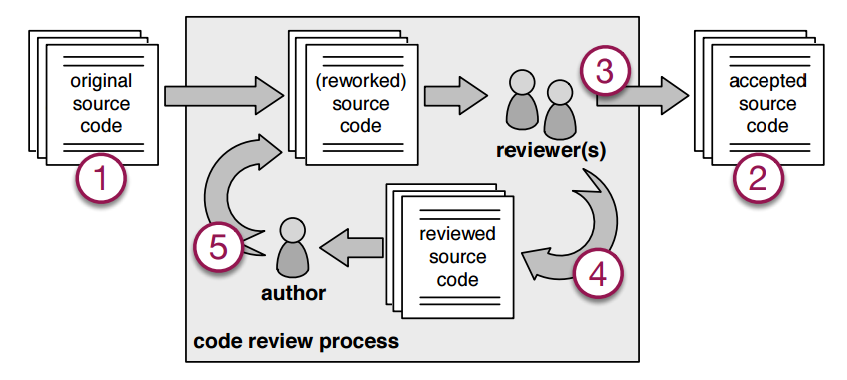
\includegraphics[width=0.75\textwidth]{images/review-process.png}
 \caption{The modern code review process (based on~\cite{beller2014modern})}
 \label{fig:review-process}
\end{figure}

To avoid the inefficiencies in code inspections, most open-source and industrial projects adopt a lightweight, flexible code review process, which we refer to as {\em modern code review}. Figure~\ref{fig:review-process} shows the workflow of modern code review. The {\em author} first submits the {\em original source code} for review. The {\em reviewers} then decide whether the submitted code meets the quality acceptance criteria. If not, reviewers can annotate the source code with review comments and send back the {\em reviewed source code}. The author then revises the code to address reviewers' comments and send it back for further reviews. This process continues till all reviewers accept the revised code.

In contrast to formal code inspections (Fagan style), modern code review occurs more regularly and informally on small yet complete program changes. 
%Mockus et al.~studied the defects in Apache bug database and found the Apache project has a defect density comparable to proprietary software~\cite{mockus2000case}. They found that this was accomplished without a policy requiring substantial code reviews before a release. They comment that this result ``may indicate that fewer defects are injected into the code, or that other defect-finding activities such as inspections are conducted more frequently or more effectively''. 
Rigby et al.~conducted the first case study about modern code review practices in an open-source software (OSS), Apache HTTP server, using archived code review records in email discussions and version control histories~\cite{rigby2008open}. They described modern code review as ``{\em early, frequent reviews of small, independent, complete contributions conducted asynchronously by a potentially large, but actually small, group of self-selected experts.}'' As code review is practiced in software projects with different settings, cultures, and policies, Rigby and Bird further investigated code review practices in a diverse set of open-source and industrial projects~\cite{rigby2013convergent}. Despite differences among projects, they found that many characteristics of modern code review have independently converged to similar values, indicating general principles of modern code review. We summarize these convergent code review practices as following.

{\bf Modern code review occurs early, quickly, and frequently.} Traditional code inspections happen after finishing a major software component and often last several weeks. In contrast, modern code review happens more frequently and quickly around the time when program changes are committed. Rigby et al.~found that the Apache project has review intervals between a few hours to a day. Rigby and Bird also observed that most reviews are picked up within a few hours in both open-source and industrial projects, indicating that reviewers are regularly watching and performing code review.

{\bf Modern code review often examines small program changes.} In the OSS project studied by Rigby et al., the median change varies from 11 to 32 changed lines. The median change size in industrial projects is larger, e.g, 44 lines in Android, 78 lines in Chrome, but still much smaller than code inspections, e.g., 263 lines in Lucene. Such small changes also facilitate developers to constantly review changes and thus keep up-to-date with the activities of their peers. 

{\bf Modern code review is conducted by a small group of self-selected reviewers.} Traditional code inspections require a designated inspection team where each member has particular roles. However, in open-source projects, program changes and review discussions are broadcast to a large group of stakeholders (often via email). Any developer can participate and share review comments. However, Rigby et al.~found that only a small number of developers (around 15) periodically participated into code review. In industrial projects, reviews are assigned in a mixed manner---the author of the code under review adds a group of reviewer candidates and these candidates then select changes to review based on their interest and expertise. Rigby and Bird found that two reviewers found an optimal number of defects.

{\bf Modern code review is often tool-based.} There is a clear trend towards utilizing review tools to support review tasks and communication. Back in 2008, Rigby et al.~reported that code review in OSS projects was often email-based due to a lack of tool support. In 2013, Rigby and Bird found that some OSS projects and all industrial projects they studied used a review tool. More recently, popular OSS hosts such as GitHub and BitBucket have integrated lightweight review tools to assign reviewers, enter comments, and record discussions. Compared with email-based reviews and traditional inspections, tool-based reviews provide the benefits of traceability and can record implicit measures. The rise in adoption of review tools provides an indicator of success.

Although the initial purpose of code review is finding defects, recent studies find that the practices and actual outcomes are less about finding defects than expected. Bacchelli and Bird studied hundreds of review comments at Microsoft and found that only a small portion of review comments were related to defects, which were mainly about small, low-level logical issues~\cite{bacchelli2013expectations}. Rather, code review provides a spectrum of benefits to software teams, such as knowledge transfer, team awareness, and improved solutions with better practices and readability. 

\subsection{Techniques for Code Change Comprehension} 

\subsubsection{Code Review Tools} 
There is a proliferation of reviewing tools, e.g., Phabricator,\footnote{\url{http://phabricator.org}} Gerrit,\footnote{\url{http://code.google.com/p/gerrit/}} CodeFlow,\footnote{\url{http://visualstudioextensions.vlasovstudio.com/2012/01/06/codeflow-code-review-tool-for-visual-studio/}} Crucible,\footnote{\url{https://www.atlassian.com/software/crucible}} and Review Board.\footnote{\url{https://www.reviewboard.org/}} The number of companies and open-source projects using lightweight review tools is also growing.

\begin{figure}[ht]
 \centering
 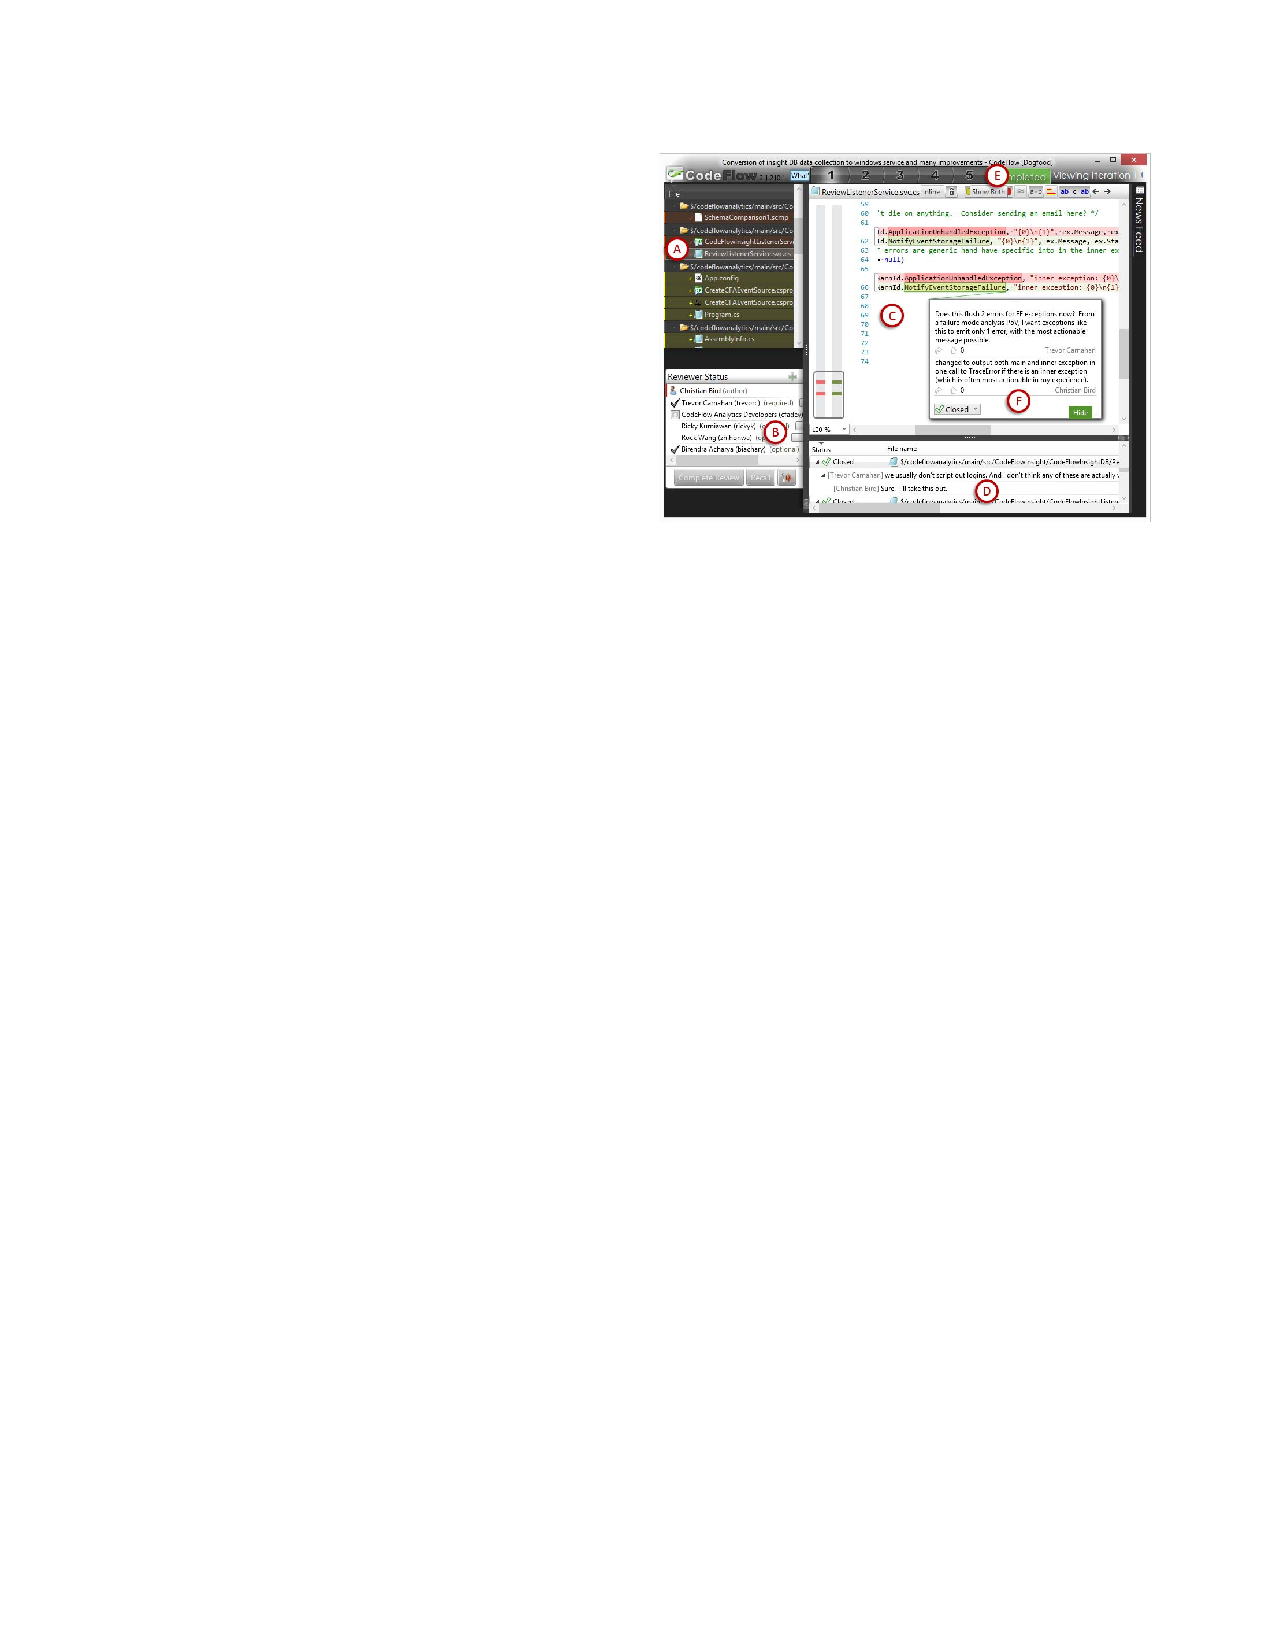
\includegraphics[width=0.75\textwidth]{images/codeflow.pdf}
 \caption{Example of code review using CodeFlow (based on~\cite{bosu2015characteristics})}
 \label{fig:codeflow}
\end{figure}

Code review tools facilitates review tasks and communications. However, change comprehension still remains a key challenge in modern code review. According to the outcomes they want to achieve, developers employ many mechanisms to fulfill their understanding needs, most of which are not currently met by any code review tool.

\subsubsection{Interactive Code Review using Change Patterns}

\subsubsection{Change Decomposition}

\subsubsection{Refactoring-aware Code Review}

% RefFinder  - extracting refactoring and showing them 
%Template-based Reconstruction of Complex Refactorings, Kyle Prete, Napol Rachatasumrit, Nikita Sudan, and Miryung Kim, ICSM '10: Proceedings of the 26th IEEE International Conference on Software Maintenance, Pages 1-10,  Publisher: IEEE DOI, presentation (local pdf) 

%Ref-Finder: a Refactoring Reconstruction Tool based on Logic Query Templates, Miryung Kim, Matthew Gee, Alex Loh, and Napol Rachatasumrit, FSE' 10: Proceedings of the 18th ACM SIGSOFT Symposium on the Foundations of Software Engineering, Pages 371-372, Publisher: ACM DOI, Formal Research Demonstration (local pdf)  

% Refactoring Inspection Support for Manual Refactoring Edits, Everton L.G. Alves, Myoungkyu Song, Tiao Massoni, Patricia D. L. Machado, Miryung Kim, TSE: IEEE Transactions on Software Engineering, 20 pages (Accepted, March 2017) (link) 

\subsection{Program Differencing} 
program differencing (going to back history of differencing, diff, AST diff, CFG diff, PDG diff.--- mention its symmetric problem of clone detection)
go deeper for a few techniques that help with change comprehension: kim et al. critics, chris bird at MS

\begin{comment}

Additional code review practice papers. 

@inproceedings{rigby2011understanding,
  title={Understanding broadcast based peer review on open source software projects},
  author={Rigby, Peter C and Storey, Margaret-Anne},
  booktitle={Proceedings of the 33rd International Conference on Software Engineering},
  pages={541--550},
  year={2011},
  organization={ACM}
}

@article{rigby2012contemporary,
  title={Contemporary peer review in action: Lessons from open source development},
  author={Rigby, Peter and Cleary, Brendan and Painchaud, Frederic and Storey, Margaret-Anne and German, Daniel},
  journal={IEEE software},
  volume={29},
  number={6},
  pages={56--61},
  year={2012},
  publisher={IEEE}
}

@article{mcintosh2016empirical,
  title={An empirical study of the impact of modern code review practices on software quality},
  author={McIntosh, Shane and Kamei, Yasutaka and Adams, Bram and Hassan, Ahmed E},
  journal={Empirical Software Engineering},
  volume={21},
  number={5},
  pages={2146--2189},
  year={2016},
  publisher={Springer}
}

\todo{The following text should be placed under code review practices: describe what are the common characteristics of modern code review processes}. 

Prior work also observes that developers often submit program changes from multiple programming tasks (e.g., bug fixing, refactorings, feature additions) to a single code review. Reviewers sometimes use ``chunky changes'' or ``code bombs'' to describe such large, unrelated changes that are bundled in a single review. Such changes often lead to difficulty in change comprehension, since reviewers have to mentally ``untangle'' them to figure out which subset of changes addresses which issue first~\cite{kawrykow2011non, murphy2012we, herzig2013impact}. Reviewers have indicated that they can better understand small, cohesive changes rather than large, tangled ones~\cite{rigby2008open}. For example, a code reviewer commented on Gson revision 1154 saying ``I would have preferred to have two different commits: one for adding the new {\ttt getFieldNamingPolicy} method, and another for allowing overriding of primitives.''\footnote{\url{https://code.google.com/p/google-gson/source/detail?r=1154}} This motivates the need of decoupling composite changes in a large code review. 

\todo{Talk about the practice of code reviewer recommendation}

Prior studies also show that a developer’s expertise on a certain part of the source code is an important factor for the effectiveness of code review tasks. However, it is not easy to determine who has the most expertise given a particular code change to review. In other words, who should review the change?

Balachandran termed the task of identifying the most appropriate reviewers for a change as {\em Reviewer Recommendation}.

@inproceedings{balachandran2013reducing,
  title={Reducing human effort and improving quality in peer code reviews using automatic static analysis and reviewer recommendation},
  author={Balachandran, Vipin},
  booktitle={Software Engineering (ICSE), 2013 35th International Conference on},
  pages={931--940},
  year={2013},
  organization={IEEE}
}

reviewer recommendation techniques 

@article{zanjani2016automatically,
  title={Automatically recommending peer reviewers in modern code review},
  author={Zanjani, Motahareh Bahrami and Kagdi, Huzefa and Bird, Christian},
  journal={IEEE Transactions on Software Engineering},
  volume={42},
  number={6},
  pages={530--543},
  year={2016},
  publisher={IEEE}
}


other expertise recommendation techniques 

@inproceedings{anvik2006should,
  title={Who should fix this bug?},
  author={Anvik, John and Hiew, Lyndon and Murphy, Gail C},
  booktitle={Proceedings of the 28th international conference on Software engineering},
  pages={361--370},
  year={2006},
  organization={ACM}
}


\todo{Talk about the code review practices and challenges in pull-based integration}
@inproceedings{gousios2015work,
  title={Work practices and challenges in pull-based development: the integrator's perspective},
  author={Gousios, Georgios and Zaidman, Andy and Storey, Margaret-Anne and Van Deursen, Arie},
  booktitle={Proceedings of the 37th International Conference on Software Engineering-Volume 1},
  pages={358--368},
  year={2015},
  organization={IEEE Press}
}

expertise assignment
Audris Mockus

\subsection{Techniques for Code Change Comprehension} 
\todo{Tianyi: Make one of the commercial code review tools a little bit more concrete and go deeper with screen shots. the following text seems like it was just copied from the intro of critics paper.}

Code review is effective only when reviewers are able to understand the changes being made. When the information required to inspect code changes is distributed across multiple files, developers find it difficult to inspect code changes~\cite{dunsmore2000object}. For example, when an API gets modified in the latest release, all call sites using this API must be updated correctly. Such edits tend to be systematic\textemdash involving similar but not identical edits to multiple locations.



\todo{For example, take a snapshot of CodeFlow or Code Collaborator, describe the tool's feature in more detail. target length should be 1 page including a screenshot.}  
Unfortunately, popular code review tools\textemdash Facebook's {\phabricator},\footnote{\url{http://phabricator.org}} Google's {\gerrit},\footnote{\url{http://code.google.com/p/gerrit/}} and Microsoft's {\codeflow},\footnote{\url{http://visualstudioextensions.vlasovstudio.com/2012/01/06/codeflow-code-review-tool-for-visual-studio/}}\textemdash all compute program differences per file. This obliges reviewers to read changed lines file by file, even when those cross-file changes are done systematically to address the same issue. Therefore, reviewers are left to manually inspect individual edits to answer questions such as ``what other code locations are changed similar to this change?'' and ``are there any other locations that are similar to this code but are not updated?''

\todo{This paper gives a very good walk-through of CodeFlow at Microsoft.}

@inproceedings{bosu2015characteristics,
  title={Characteristics of useful code reviews: An empirical study at microsoft},
  author={Bosu, Amiangshu and Greiler, Michaela and Bird, Christian},
  booktitle={Mining Software Repositories (MSR), 2015 IEEE/ACM 12th Working Conference on},
  pages={146--156},
  year={2015},
  organization={IEEE}
}


\subsubsection{Interactive Code Review using Code Patterns} 
\todo{Right now there's too much focus on Critics. Reduce the length to be 1.5 pages including a screen snapshot.}
\begin{figure}[ht]
 \centering
 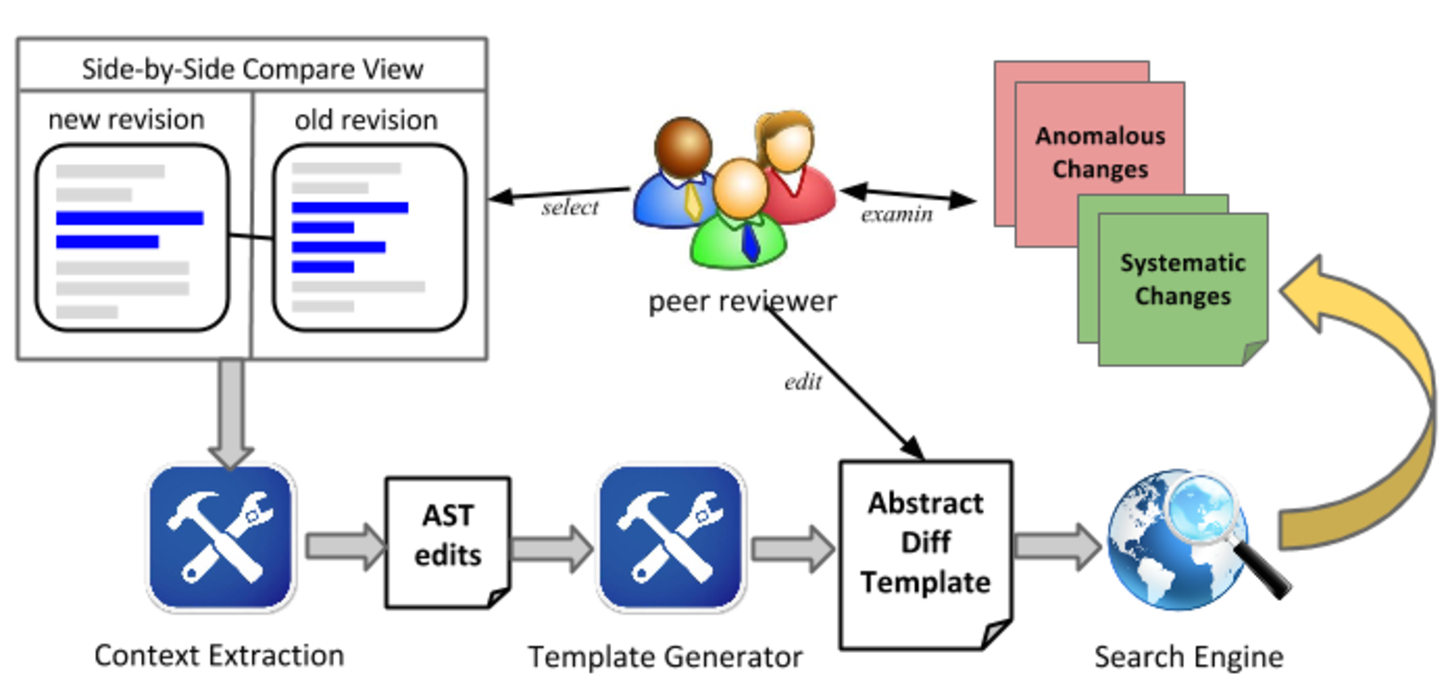
\includegraphics[width=0.8\textwidth]{images/critics-workflow.pdf}
 \caption{The workflow of {\critics}}
 \label{fig:critics-workflow}
\end{figure}

To address this issue, Zhang et al.~present {\critics}, a novel approach that allows reviewers to interactively inspect such systematic changes during peer code review~\cite{zhang2015interactive}. Figure~\ref{fig:critics-workflow} describes the interactive workflow of {\critics}. Given a specified change that a reviewer would like to inspect, {\critics} creates a change template from the selected change, which serves as the pattern for searching similar changes. {\critics} includes {\em change context} in the template---unchanged, surrounding program statements that are relevant to the selected change. {\critics} models the template as Abstract Syntax Tree (AST) edits and allows reviewers to iteratively customize the template by parameterizing its content and by excluding certain statements. {\critics} then matches the customized template against the rest of the codebase to summarize similar changes and locate potential inconsistent or missing changes. Reviewers can incrementally refine the template and progressively search for similar changes until they are satisfied with the inspection results. This interactive feature allows reviewers with little knowledge of a codebase to flexibly explore the program changes with a desired pattern.



\begin{figure}[ht]
 \centering
 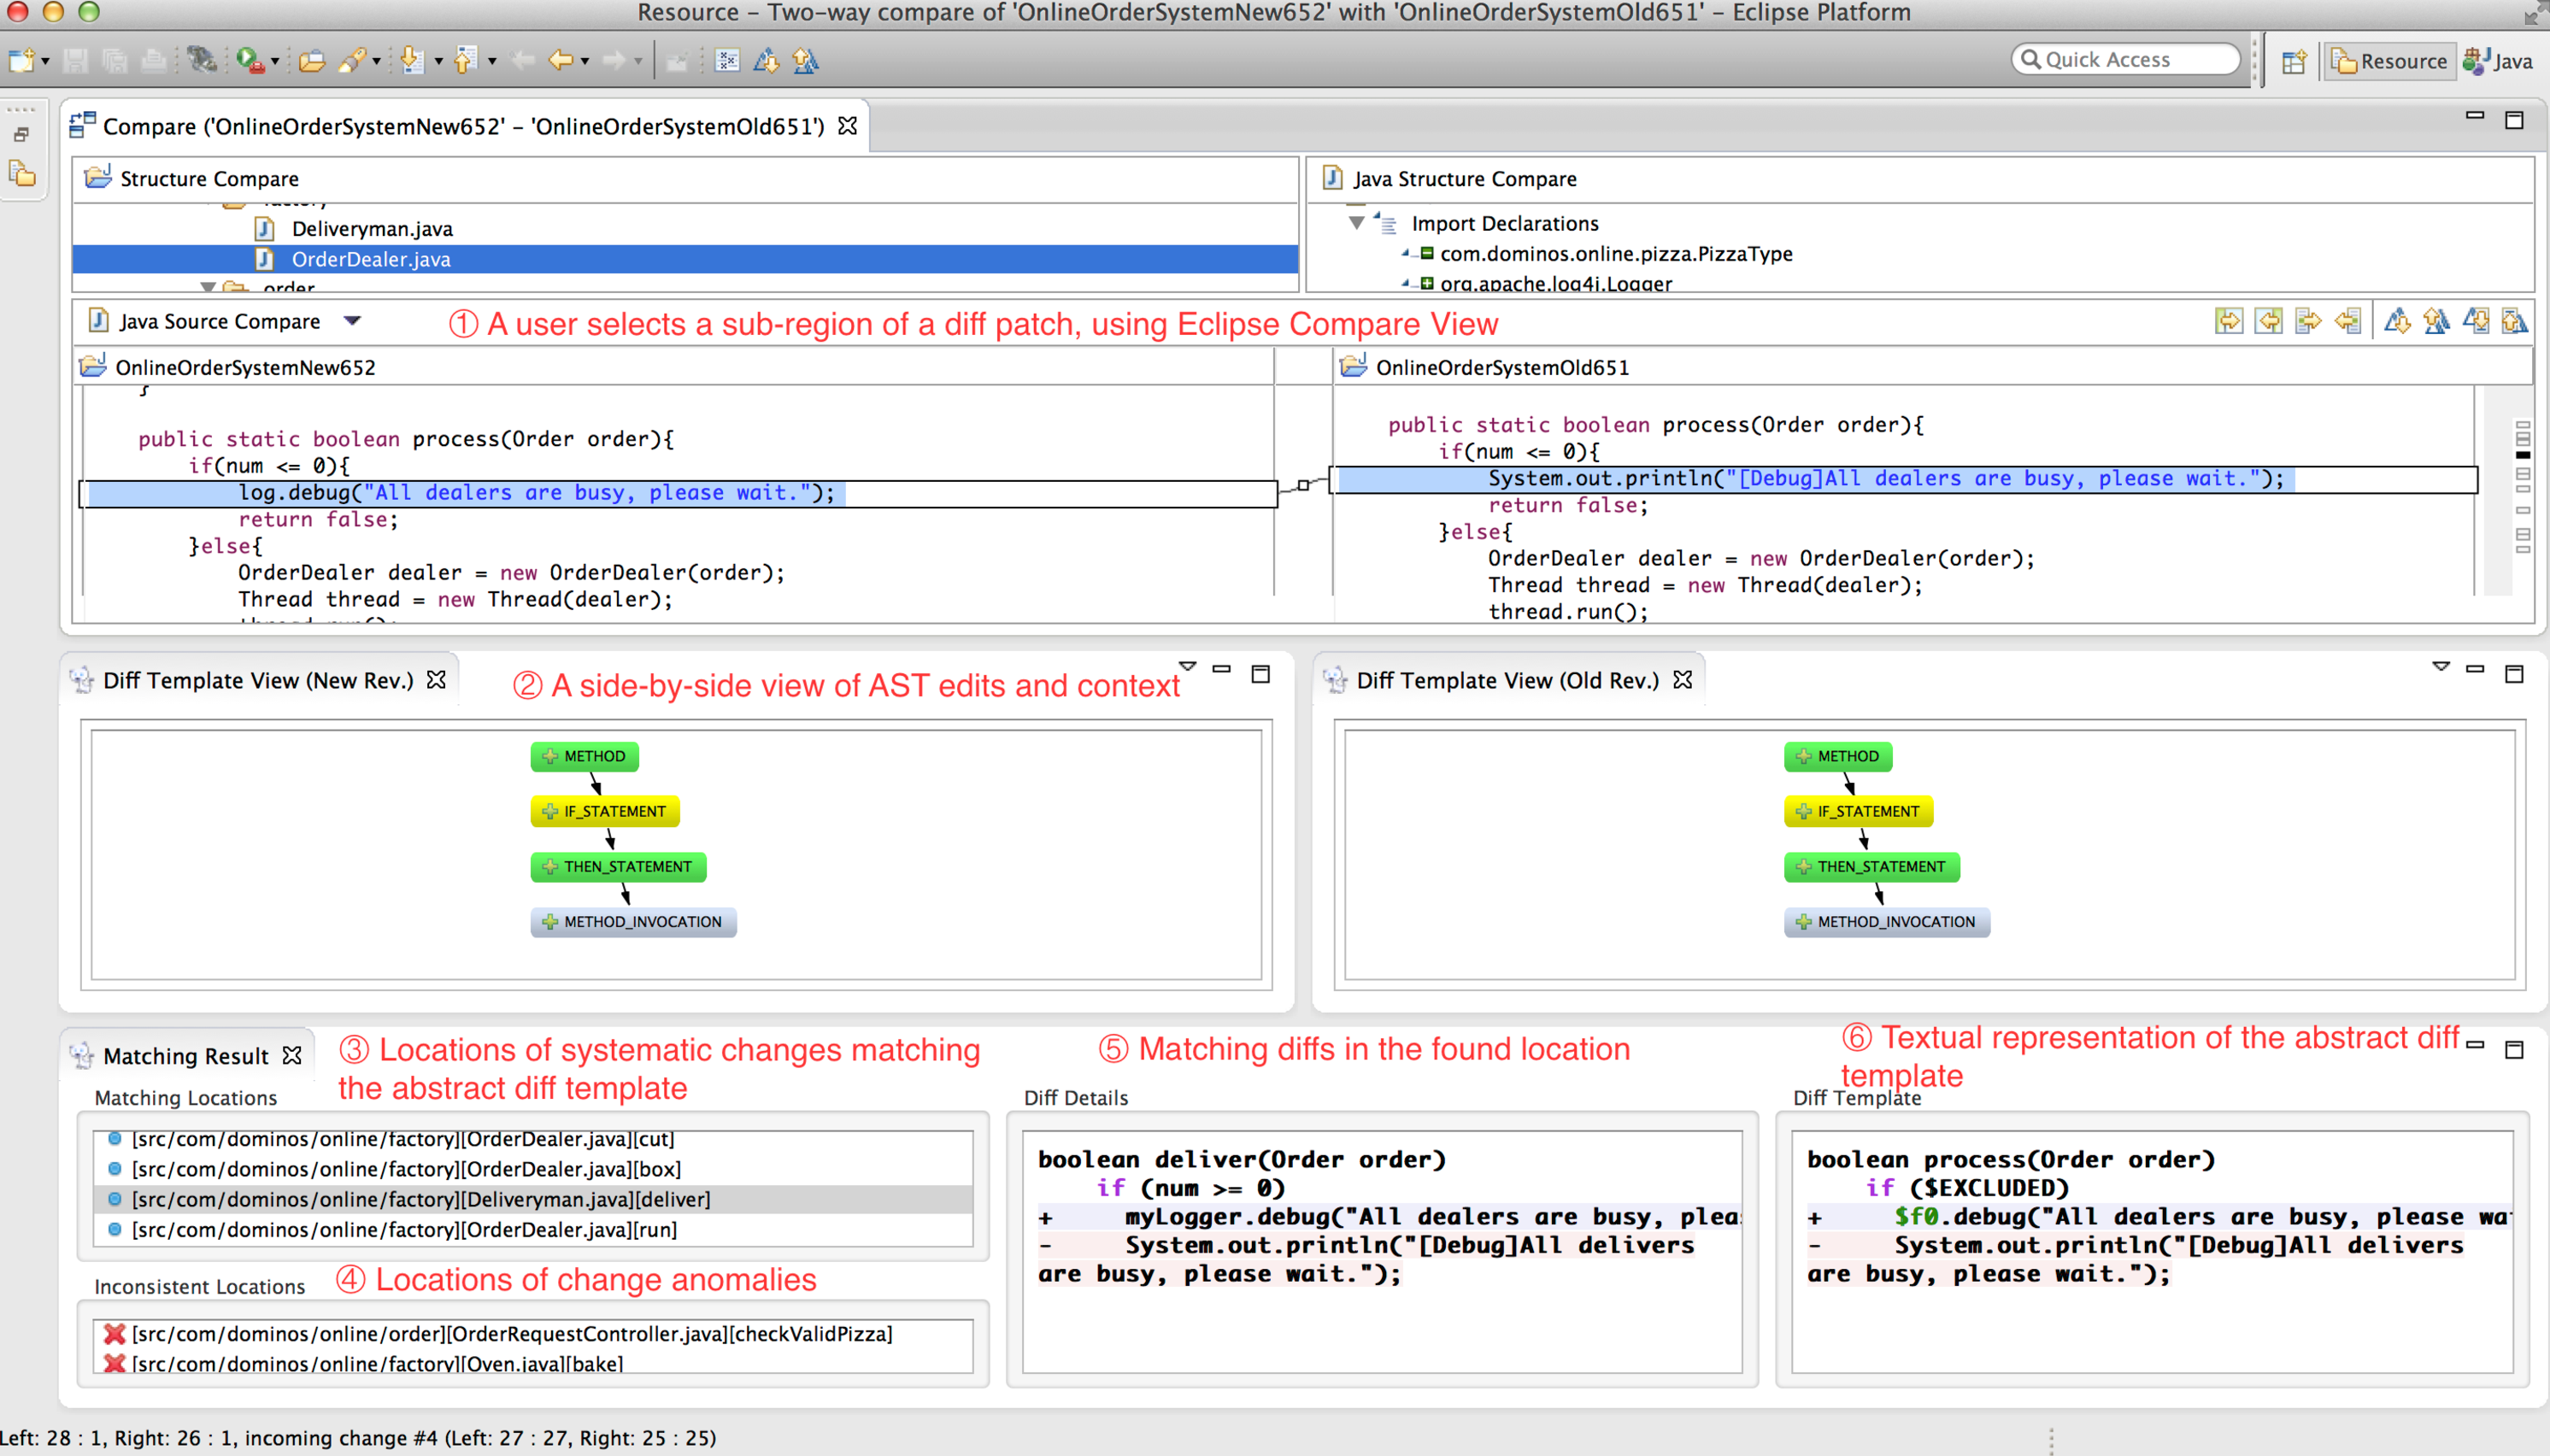
\includegraphics[width=\textwidth]{images/critics-UI.pdf}
 \caption{A screen snapshot of {\critics}'s Eclipse plugin and its features}
 \label{fig:critics-UI}
\end{figure}

{\critics} is implemented as an Eclipse plugin.\footnote{{\critics}'s tool and evaluation dataset are available online \url{https://sites.google.com/a/utexas.edu/critics/}} Figure~\ref{fig:critics-UI} shows a screenshot of {\critics} plugin. {\critics} is integrated with the {\bf Compare View} in Eclipse, which displays line-level differences per file (see \ding{172} in Figure~\ref{fig:critics-UI}). A user can specify a program change she wants to inspect by selecting the corresponding code region in the Eclipse Compare View. The {\bf Diff Template View} (see \ding{173} in Figure~\ref{fig:critics-UI}) visualizes the change template of the selected change in a side-by-side view. Reviewers can parameterize concrete identifiers and exclude certain program statements by clicking on the corresponding node in the Diff Template View. {\bf Textual Diff Template View} (see \ding{177} in Figure~\ref{fig:critics-UI}) shows the change template in a unified format. The {\bf Matching Result View} summarizes the consistent changes as {\em similar changes} (see \ding{174} in Figure~\ref{fig:critics-UI}) and inconsistent ones as {\em anomalies} (see \ding{175} in Figure~\ref{fig:critics-UI}).


\todo{the evaluation and quotes are too much for this chapter. so I removed them} 
\subsubsection{Change Decomposition} 
 
\todo{ make the length less than 1 page in total} 

To address this issue, Barnett et al.~present {\clusterchanges}, a lightweight static analysis technique for decomposing large changes. The insight is that program changes that address the same issue can be related via implicit dependency information such as {\em def-use} relationship. For example, if a method definition is changed in one location and its callsites are changed in two other locations, these three changes are likely to be related and should be reviewed together. Given a code review task, {\clusterchanges} first collects the set of definitions for types, fields, methods, and local variables in the corresponding project under review. Then {\clusterchanges} scans the project for all uses (i.e., references to a definition) of the defined code elements. For instance, any occurrence of a type, field, or method either inside a method or a field initialization is considered to be a use. Based on the extracted def-use information, {\clusterchanges} identifies three relationships between program changes. 

\todo{Remove a bullet list and integrate into text.}
\begin{itemize}
 \item {\bf Def-use relation}. If the definition of a method or a class field is changed, all the uses should also be updated. The change in the definition and the corresponding changes in its references are considered related.
 \item {\bf Use-use relation}. If two or more uses of a method or a class field defined within the change-set are changed, these changes are considered related. 
 \item {\bf Enclosing relation}. Program changes in the same method are considered related because a) based on observation, program changes to the same method are often related, (b) reviewers often inspect methods atomically rather than reviewing different changed regions in the same method separately.
\end{itemize}

Given these relations, {\clusterchanges} creates a partition over the set of program changes by computing a transitive closure of related changes. On the other hand, if a change is not related to any other changes, it will be put into a specific partition, {\em miscellaneous changes}.

\todo{Expand the following technique a little bit more. Give similar weights to ClusterChange.}
Independently from {\clusterchanges}, Tao et al.~present a similar change decomposition technique that leverages more sophisticated heuristics, other than the def-use analysis only~\cite{tao2015partitioning}. Tao et al.~cluster changes based on the following heuristics.

\subsubsection{Refactoring Aware Code Review} 

% RefFinder  - extracting refactoring and showing them 
%Template-based Reconstruction of Complex Refactorings, Kyle Prete, Napol Rachatasumrit, Nikita Sudan, and Miryung Kim, ICSM '10: Proceedings of the 26th IEEE International Conference on Software Maintenance, Pages 1-10,  Publisher: IEEE DOI, presentation (local pdf) 

%Ref-Finder: a Refactoring Reconstruction Tool based on Logic Query Templates, Miryung Kim, Matthew Gee, Alex Loh, and Napol Rachatasumrit, FSE' 10: Proceedings of the 18th ACM SIGSOFT Symposium on the Foundations of Software Engineering, Pages 371-372, Publisher: ACM DOI, Formal Research Demonstration (local pdf)  

% Refactoring Inspection Support for Manual Refactoring Edits, Everton L.G. Alves, Myoungkyu Song, Tiao Massoni, Patricia D. L. Machado, Miryung Kim, TSE: IEEE Transactions on Software Engineering, 20 pages (Accepted, March 2017) (link) 

\subsection{Program Differencing} 
program differencing (going to back history of differencing, diff, AST diff, CFG diff, PDG diff.--- mention its symmetric problem of clone detection)
go deeper for a few techniques that help with change comprehension: kim et al. critics, chris bird at MS


\end{comment} 
\section{An Organized Tour of Seminal Papers: III. Change Validation} 
\label{sec:debugtest}

\begin{figure}[ht]
 \centering
 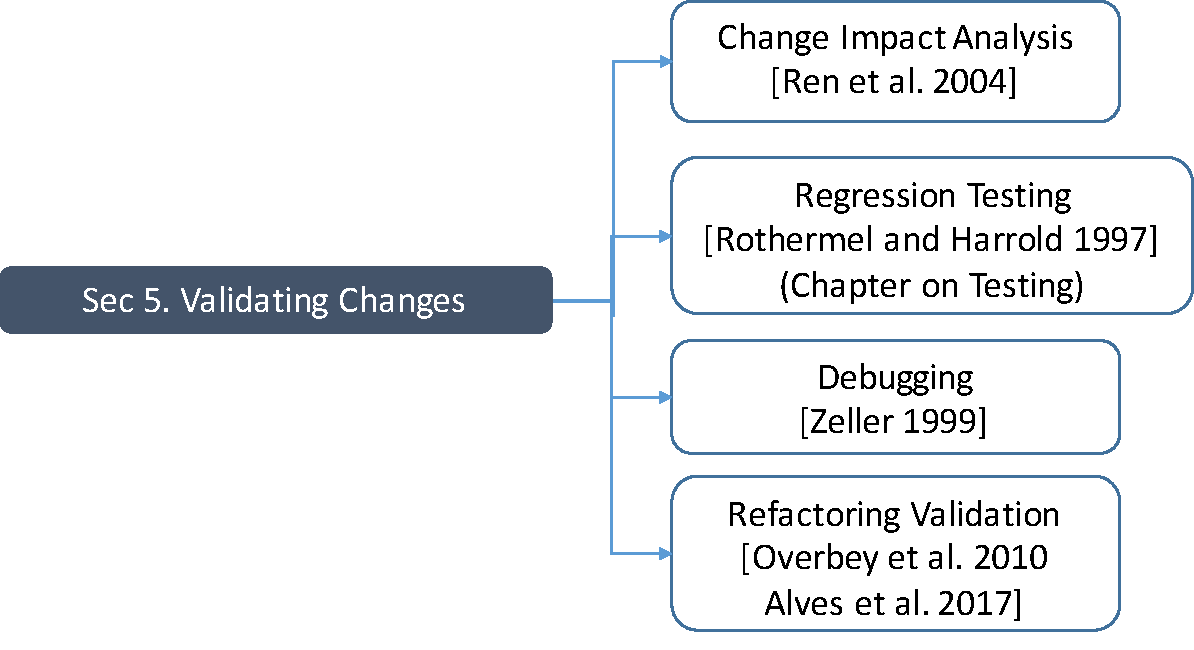
\includegraphics[width=0.6\textwidth]{images/ChangeValidation.pdf} 
 \caption{Change Validation and Related Research Topics} 
 \label{fig:changevalidation} 
\end{figure}



\subsection{Delta Debugging: Finding Code Changes Causing Errors}
\todo{2 pages} 
\subsection{Regression Testing} 
\todo{2 pages} 
\paragraph{Change Impact Analysis} 
\todo{2 pages} 

\section{Future Directions and Open Problems} 
\todo {4 pages} 


\subsubsection*{Acknowledgments.} The heading should be treated as a
subsubsection heading and should not be assigned a number.

\section{The References Section}\label{references}
\bibliography{tianyi,mengna,reference,miryung}
\bibliographystyle{abbrv}

\section*{Appendix} 
\end{document}
